\documentclass[11pt,titlepage]{article}
\usepackage[utf8]{inputenc}
\usepackage[letterpaper, total={6.5in, 9in}]{geometry}

\title{Machine Learning-Based Reconstruction of Neuronal Networks from Calcium Imaging Signals}
\author{Derek Low}
\date{2017 - 2018}

\usepackage{setspace}
\usepackage{floatrow}
\usepackage{fancyhdr}
\usepackage{multirow}
\usepackage{natbib}
\usepackage{graphicx}
\usepackage{upgreek}
\usepackage{amsmath}
\usepackage{float}
\usepackage{mwe}
\usepackage{subfig}
\usepackage[font={scriptsize,stretch=1.6},labelfont=bf]{caption}
\captionsetup{justification   = raggedright,
              singlelinecheck = false}
\renewcommand{\baselinestretch}{1.6}
\usepackage[ruled,vlined]{algorithm2e}
\DontPrintSemicolon
\newcommand{\To}{\mbox{\upshape\bfseries to}}

\fancyhf{}
\fancyhead[C]{\thepage}
\pagestyle{fancy}

\fancyhf{}
\fancyhead[C]{\thepage}
\setlength{\headheight}{40pt}


\begin{document}
\pagenumbering{gobble}
\begin{titlepage}
    \begin{center}
        \vspace*{1cm}
        
        \Huge
        \textbf{Machine Learning-Based Reconstruction of Neuronal Networks from Calcium Imaging Signals}
        
        \vspace{0.5cm}
        
        \vspace{1.5cm}
        \LARGE
        \textbf{Derek Low}
        
        \vspace{5cm}
        \Large
       	A Senior Project Submitted to\\
       	The Division of Science, Mathematics, and Computing\\
       	of Bard College
        
        \vspace{0.8cm}
        
        \Large
        Annandale-On-Hudson, New York\\
        2017-2018
        
    \end{center}
\end{titlepage}
\clearpage
\subsection{Brief Description}
Activity of neuronal networks can be recorded via Calcium Imaging. In this study, we develop a machine learning approach to reconstructing network connectivity from calcium imaging data.

\subsection{Abstract}
%expand on why "structural neuronal network connectivity" is important
%expand on why its difficult
%missing results section (final sentences)
%take some of the jargon out and boil it down to the essense in "we develop a model...""we update..."
%3rd sentence -> use NEST to simulate connectivity, create spiking data, use machine learning to predict our initial connectivity. THEN you can have the "we develop a model"
One of the major areas of research in computational neuroscience is focused on relating the connections within populations of neurons to the signaling activity of these populations. Methods of reconstructing structural neuronal network connectivity are limited and, in large populations, technically infeasible. Current methods that reconstruct networks of large populations relate connectivity to calcium imaging recordings of these networks. Here, we introduce a machine-learning approach to inferring connectivity from spike-time data extracted from calcium imaging recordings. First, we simulate populations of neurons with the NEST simulator to produce downsampled spike-trains. We develop a model based on neural networks, which is a widely applied machine-learning method. The model is updated with gradient descent on the error via backpropagation, and the performance is compared to the widely used cross-correlation method of extracting functional connectivity. We then train the models on simulated data and \textit{in-vivo} calcium imaging data from \textit{Xenopus Laevis} tadpoles.

\clearpage
\section*{Dedications and Acknowledgements}
I thank Professor Arseny Khakhalin of the Bard College Biology Department and Professor Kerri-Ann Norton of the Bard College Computer Science Department for dedicating their time and effort to advising on all aspects of this senior project. Without their constant support and encouragement, there would be no project. Throughout the course of this project, I have  encountered many of my own shortcomings, and I truly thank my two senior project advisors in assisting me through overcoming these shortcomings, and, furthermore, through the difficult moments of the project.\par
I thank my various professors and colleagues throughout the four years of my education at Bard, for encouraging my academic growth in all avenues of learning.\par
I thank my dearest friends for their constant encouragement throughout the senior project, and throughout my senior year. Thank you for realizing my potential in my moments of deepest insecurity. Thank you for demonstrating to me the vast possibilities and moments for happiness that exist in every day, no matter how I may be feeling.\par
I thank the Bard Swimming Team, as their captain for two years, and as their teammate and swimmer for four. True dedication comes without expectation of reward, but these past four years have been nothing but a reward with my amazing teammates.\par
I thank my parents, for loving and caring for me, and encouraging me throughout the senior project process, and throughout my education at Bard College. Their support and love, lacking any expectation or condition, is something I can never repay, and can never appreciate enough.\par
I thank my sister, for being completely extra, and for reminding me of what it is to be human.\par
I thank my partner, Mary Grace McNulty, for her constant confidence in me, and for being simultaneously calming and breathtaking. Mary, thank you for being the comforting and jubilant presence in my life.\par
\clearpage
\tableofcontents
\clearpage
\listoffigures
\clearpage
\pagenumbering{arabic}
\section{Introduction}
\setcounter{page}{1}
\subsection{The Neuron}\label{ssec:Neuron}
Neurons are fundamental to human cognition, and encode for a large range of activities such as movement, speech, and decision making. The interactions between neurons throughout the human body have been studied at microscopic levels, with focus on the specific mechanisms and dynamics of molecules within neurons that allow for propagation of signals from one neuron to the next neuron (Bean, 2007). Networks of neurons have also been studied at macroscopic levels, relating specific regions to distinct functions, such as the relationship between the brain and human capabilities of cognitive control and activity, or the specific activity of particular regions of the brain (Biswal et al., 1995; Mazzoni et al., 2007). However, the precise connectivity patterns of neurons, and the relationship between this organization and its possible functions, are not fully understood (Bock et al., 2011). Interpreting the patterns of connections in neuronal populations as networks of nodes provides a foundation for characterizing network properties and studying statistical features of these populations. Additionally, understanding these connections and network characteristics may provide insight to the function and activity of these populations of neurons, and imply a relationship between functional and structural connectivity.\par

%Neurons are fundamental to human cognition, and encode for a large range of activities such as movement, speech, decision making, and learning among many other functions in the human body. The interactions between neurons throughout the human body are studied at microscopic levels; such studies may concern the signal propagation along neurons in the hippocampus (Hoffman et al., 1997), or the dynamics of the synapse, the structure of connection between neurons, and implications of changes to those dynamics (Haydon, 2001; Terry et al., 1991). Additionally, networks of neurons are studied at macroscopic levels, where certain regions of the brain are responsible for certain functions of the body, such as the relationship between the prefrontal cortex and human capabilities of cognitive control and activity (Miller and Cohen, 2001), or sensorimotor cortex activity and the resulting motor imagery and action (Porro et al., 1996). However, the precise connectivity patterns of neurons, and the relationship between this organization and its possible functions, are not fully understood. Analysis of the patterns of connections in populations of neurons indicate that these cells are characterized by certain network properties. Therefore, understandings of these connections may provide insight to the function and activity of these populations of neurons, and possible implications of a relationship between functional and structural connectivity.\par


%include something here to talk about what a "potential" is?
The transmission of signals within parts of neurons is partially mediated by the electrical potential difference between a neuron and its surrounding environment, known as the membrane potential. The earliest and most influential studies concerning the effects of ions in neurons were conducted by Hodgkin, Huxley, and Katz nearly 70 years ago, and clearly indicated the relationship between ion concentration and the activity of neurons. Giant squid axons in lower sodium environments maintained a lower resting potential, as well as a weaker and delayed action potential (Hodgkin and Katz, 1949). 
%Perhaps word this a little differently?
Changes in concentrations of ions, distributed in varying concentrations throughout the nervous system, mediate neuron activity by changing this membrane potential. In a state of low activity, this membrane defaults to a polarized state of negative electrical potential, referred to as the resting membrane potential (Purves et al. pp.31, 2004,). When the membrane potential moves in the positive direction, signal propagation along the neuron occurs.\par

Communication between neurons occurs at the synapse, a structure of connection between two neurons. The communication occurs via a synaptic potential, a signal from the pre-synaptic to the post-synaptic neuron, and is initiated by the release of neurotransmitters from the presynaptic neuron that interact with receptors in the postsynaptic neuron. Synaptic potentials are either excitatory, increasing the membrane potential of the neuron towards positive values (depolarization), or inhibitory, reducing potential towards negative values (hyperpolarization) (Bean, 2007; Armstrong and Hille, 1998). The resulting depolarization due to the excitatory post-synaptic potentials (EPSPs) increases the membrane potential towards higher positive values, until a specific threshold is reached (Bean, 2007). Once a specific depolarization threshold is reached, an action potential is generated, and propagates along the neuron until it reaches another synapse, at which point the cycle of neurotransmitter release, synaptic potential, and action potential propagation cycle may be repeated (Bean, 2007).\par

%The earliest and most influential studies concerning the effects of ions in neurons were conducted by Hodgkin, Huxley, and Katz nearly 70 years ago, and clearly indicated the impact of sodium concentration on the activity of neurons; giant squid axons in lower sodium environments demonstrated a lower resting potential, as well as a weaker and delayed action potential (Hodgkin and Katz, 1949). Potassium concentration demonstrates a similar impact to the membrane potential, with a reduced concentration resulting in higher resting and action potentials and a shallower repolarization of the membrane (Hodgkin and Katz, 1949). Membrane potential is quantified by the polarity of these ionic molecules, and their respective concentrations on each side of the membrane, or the difference between the intracellular and extracellular concentrations of the ion.\par

The propagation of action potentials involves constant changes to the electrochemical gradients of the neurons by the opening and closing of ion channels in the membrane. The ion channels involved in generating action potentials, mediating and raising membrane potentials towards distinct states of polarization during neuronal signaling include the voltage-gated ion channels, specifically the sodium (Na\textsuperscript{+}), potassium (K\textsuperscript{+}) and calcium (Ca\textsuperscript{2+}) channels. However, while these channels serve similar purposes of allowing passage of certain ions and restricting passage of other ions, the time of activation of each type of channel establishes their distinct impacts on propagation (Purves, 2004, 76-78). The depolarization of the neuron, and consequent upswing in membrane potential towards positive values, is caused by the influx of sodium from the extracellular medium into the cell; this influx is caused by the opening of sodium channels following an EPSP, prior to the membrane potential reaching the threshold potential and the initiation of an action potential. (Hodgkin and Katz, 1949; Hodgkin and Huxley, 1952). The resulting repolarization and hyperpolarization stages preceding the return to resting membrane potential result from the efflux of potassium; this efflux is a delayed response to the initiation of the action potential, indicating a delayed opening of potassium channels following the opening of sodium channels (Hodgkin and Huxley, 1952). This change in membrane potential is the mechanism of signal propagation, and is referred to as the action potential, or the neuronal \textit{spike}, and is the primary method of observing neuronal activity in neuroscience research.\par

\subsection{Calcium Imaging}
%A commonly employed method of recording activity of neurons is calcium imaging. Neuron activity. At every spiking event, these ions travel through the cell membrane of each neuron by movement through voltage-dependent ion channels, which are functionally altered by the voltage changes that occur in neurons.\par

One method of recording neuronal activity across populations of neurons is calcium imaging. In most mammilian neurons, the intracelluar calcium concentration is about 50-100 nM, and can rise to levels during of 10 to 100 times higher during neuronal activity (Grienberger and Konnerth, 2012; Berridge et al., 2000). Calcium performs several major roles in the function and management of biological cells; most notably, in the presynaptic neuron, an influx of calcium into the neuron triggers the release of neurotransmitter to the synapse via exocytosis (Katz and Miledi, 1967). Furthermore, presynaptically, residual calcium results in neural facilitation, a period in which a successive depolarization of the presynaptic neuron, following the first depolarization event and release of neurotransmitter, raises the likelihood of neurotransmitter release (Katz and Miledi, 1967; Zucker, 1999). Postsynaptically, calcium is responsible for activating the synaptic plasticity cascade. These changes to the synapse involve the influx of calcium through the N-methyl-D-aspartate receptor (NMDA) and $\alpha$-amino-3-hydroxy-5-methyl-4-isoxazolepropionic acid receptor (AMPA), result in changes to the sensitivity of the neuron and, by extension, the interactions between the pre- and postsynaptic neurons (Zucker, 1999). The changes enhance or diminish the strength of the connection (potentiation and depression), in various temporal manners (short and long-term). For example, in the case of long-term potentiation (LTP), the influx of calcium into the postsynaptic neuron, and the resulting depolarization, result in the unblocking of the NMDA receptors, allowing for a further influx of calcium into the postsynaptic neuron and inducing LTP (Zucker 1999).Functions of calcium extend further than synaptic activity, and the ion is additionally responsible for biological functions such as cell apoptosis (Orrenius et al., 2003). Therefore, the abundance and utility of calcium, and the deeply integral relationship between calcium and neuron activity, suggest it to be a strong candidate for the purpose of imaging the activity of neuronal populations.\par

\subsubsection{Calcium Indicators}
As mentioned, calcium influx to the neuron depends on changes in the membrane potential of neurons, and the responses of voltage-gated channels during neuron activity. Concentration of calcium is higher extracellularly until spike time. During neuron activity, the influx of calcium results in the release of synaptic vesicles containing neurotransmitters (Grienberger and Konnerth, 2012). Therefore, introducing an indicator that fluoresces when bound to calcium allows recording of calcium concentration and activity. Among the first discovered and applied calcium indicators is the protein aequorin (Shimomura et al., 1962), where the binding of the calcium to three binding sites located on the protein results in photon emission (Grienberger and Konnerth, 2012). The necessity of three calcium molecules, in combination with a controlled amount of indicator injected into these neurons, allows for a controlled fluorescence method that is directly related to the calcium concentration within the cell. However, the particular drawbacks of aequorin, such as a low protein stability and a relatively low fluorescence rate with regards to the amount of decomposition in the concentration of the protein, result in development of several superior and modern alternatives (Grienberger and Konnerth, 2012).\par

Modern calcium indicators are typically categorized as high-affinity or low-affinity, where high-affinity indicates the most commonly used indicators with wide varieties of application. One such high-affinity calcium indicator is fura-2 (Grynkiewicz et al., 1985); this indicator operates by excitation with ultraviolet light, resulting in a fluorescence shift of the indicator; the fluorescence level changes when the molecule is bound to calcium, a property referred to as ratiometric, dual-wavelength, or dual-excitation (Grienberger and Konnerth, 2012). This particular indicator is applied to a variety of microscopy methods, including two-photon microscopy (discussed below), requiring slight modification by inclusion of green fluorescent protein (GFP) in the latter case (Grinberger and Konnerth, 2012). 

\subsubsection{Calcium Microscopy}
The second component of calcium imaging is the imaging, recording, and approximation of recorded data as a measurement of brain activity. There are several technologies employed in the recording of calcium indicator fluorescence; the technique used widely depends on the subject being recorded and quality of the imaging required. However, an equally wide range of techniques are available, and have particular benefits and drawbacks relating to the method and observed sample.\par

All microscopy techniques result in the photobleaching and phototoxicity of the observed specimens, resulting in photodamage (Svodoba et al., 2006). Another restricting factor in microscopy is photon scattering, a process in which a photon is absorbed by a molecule and re-emitted in a distinctly random direction, resulting in the blurring of the resulting microscopy image (Ntziachristos, 2010). Therefore, one aim relevant to employed microscopy techniques is the highest accumulation of imaging data with the lowest possible amount of photodamage to the observed specimen, and lowest photon scattering for image accuracy and clarity. Prior to the development of two photon microscopy in the 1990's (Denk et al., 1990), most microscopy methods used, such as confocal and wide-field fluorescence microscopy, suffered from the major drawback of having low tissue penetration depth due to photon scattering and, in the case of confocal microscopy, tissue degradation (Svodoba et al., 2006).\par

\subsection{Xenopus Tadpoles}
The \textit{Xenopus Laevis} tadpole is an experimental model and has been used in a variety of neuronal studies, such as studies in developmental changes in responses to sensory stimuli, the role of neural activity on changes in neural circuits, and the roles of excitatory and inhibitory connections on behavioral responses (Dong et al., 2008; Khakhalin et al., 2014; Ciarleglio et al., 2015). The inputs and outputs to tadpole neuronal networks in the optic tectum can be accessed \textit{in vivo}, and electrophysiological and  calcium imaging data can be recorded from these networks (Xu et al., 2011; Khakhalin et al., 2014). Due to the ease of access to the surface of the tectum via removal of the skin around the \textit{Xenopus} tadpole skin, the optic tectum is viable target \textit{in-vivo} observation (Xu et al., 2011; Khakhalin et al., 2014)Additionally, changes in activity due to changes in sensory inputs to the eyes of the \textit{Xenopus} tadpole can be recorded \textit{in-vivo}, during stimulation (Jang et al., 2016). Therefore, the \textit{Xenopus Laevis} tadpole is a viable model for research concerning the relationship between distinct neuronal patterns of activity and the underlying networks.\par
For example, Xu et al., 2011 recorded large-scale neural activity via in-vivo calcium imaging to detect synchronous patterns of spiking across the population of neurons. In this study, spike trains of individual tectal neurons within a larger neuronal population were observed by recording the Ca\textsuperscript{2+} responses via a membrane-permeant Ca\textsuperscript{2+} indicator. The Ca\textsuperscript{2+} images recorded were first filtered and deconvolved, a method of reducing noise involving an algorithm to specifically reduce the imaging artifacts (Xu et al., 2011). In the case of calcium imaging, these artifacts primarily originate from the slow decays of calcium signals, and the slow decay nature restricts the imaging of spikes occurring in rapid succession. To counteract this effect, Xu et al. deconvolve calcium imaging data by selecting and loose-patch clamping a subset of tadpole tectal neurons to record the action potentials simultaneous to the calcium imaging (Xu et al., 2011). From this simultaneously recorded electrophysiological and calcium imaging data, a relationship between the more precise, smaller scale method (loose-patch clamp) and the less precise, larger scale method (calcium imaging) was calculated and applied for deconvolution of the calcium imaging signal. Analyzing the resulting deconvoluted data identified individual spike times from the signals produced by the calcium-sensitive dyes during visual stimulation (Xu et al., 2011).\par

\subsection{Representing Networks of Neurons}
The organization of neurons can be represented as a matrix, typically referred to as an adjacency or weight matrix, depending on how these connections between neurons are represented, and what information is useful and preserved. Weight matrices assign values based on the strength of connections between neurons, and whether the source neuron is an excitatory or inhibitory neuron, while adjacency matrices are representative of whether or not there is a connection, and ignores the strength of these connections. These matrices represent a graph, or network, with the connections represented by the indices of the matrix, and the nodes as the columns and rows of the matrix. For example, the following matrix describes connections between a population of three neurons in a directed graph, where all connections are unidirectional:\par
\begin{figure}[H]
\begin{center}
\begin{tabular}{ |p{3cm}|p{3cm}|p{3cm}|p{3cm}|  }
 \multicolumn{4}{}{}\\
 \hline
  & Neuron 1 & Neuron 2 & Neuron 3\\
 \hline
 Neuron 1 & 0 & 1 & 1\\
 Neuron 2 & 0 & 0 & 0\\
 Neuron 3 & 1 & 1 & 0\\
 \hline
\end{tabular}
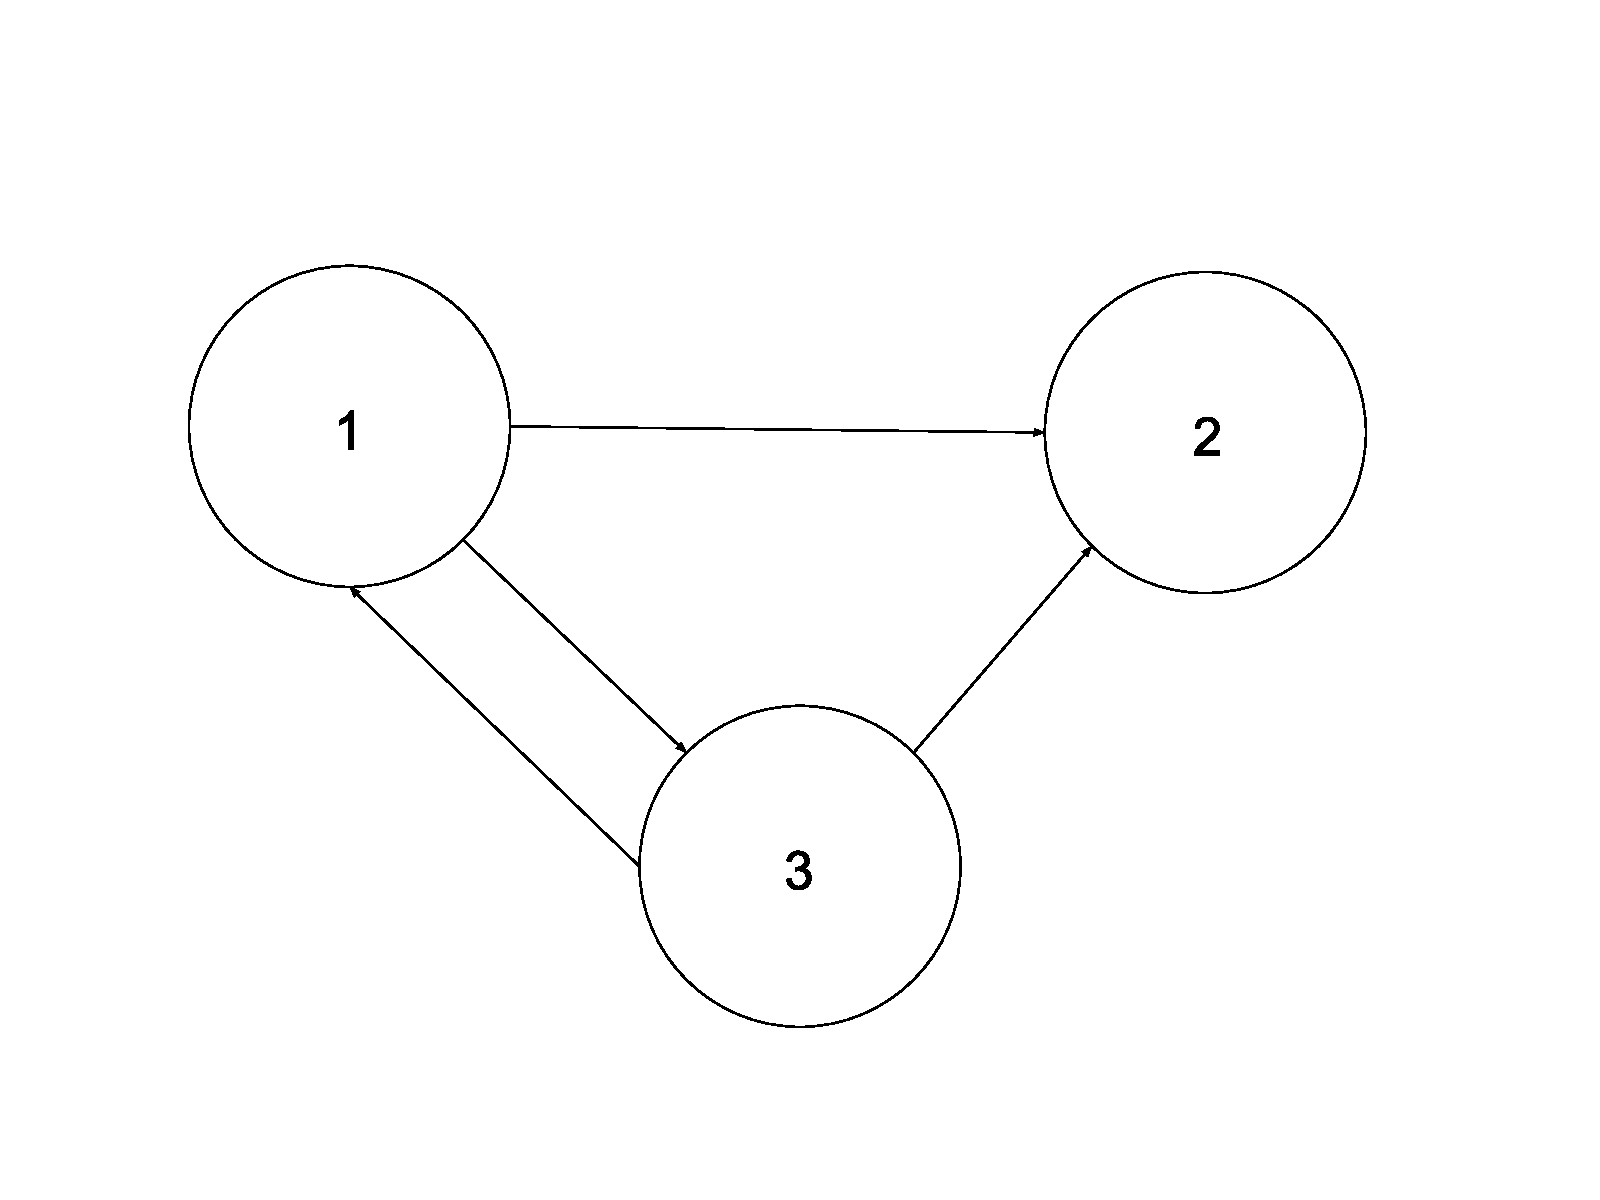
\includegraphics[scale=0.4,trim={0 2.7cm 0 3.5cm},clip]{./Figures/demonstratingConnectivity.pdf}
\end{center}
\caption[Sample Adjacency Matrix of Population Size 3]{Sample Adjacency Matrix of Population Size 3. Diagonal indices, starting from entry [1,1] and extending to entry [3,3], represent self-connections. Labels along the columns represent the target, and labels along the rows represent the source e.g. the connection at Row 3, Column 2 (value of 1) is a connection from the pre-synaptic Neuron 3 to the post-synaptic Neuron 2. Note the lack of the inverse connection from Neuron 2 to Neuron 3 (value of 0) in the directed graph depiction.}
\label{adjMatrix}
\end{figure}

Matrices such as the one above describe the connections between different neurons in an observed population; these neurons could have incoming connections from sources outside of the observed population, depending on the context of the observations. Network matrices contain a zero value along the diagonal, representative of a lack of a connection from a neuron to itself. In the example above, there is a directional connection between the outward axonal connection of Neuron 3 and the incoming dendritic connection of Neuron 1; therefore, assuming a positive value to represent an excitatory connection, spikes in Neuron 3 result in a voltage increase of Neuron 1. By this method of representation, the matrix can describe the relative strength and nature of all connections between neurons in the observed population.\par

%Currently, methods of studying neurons and brain activity rely on techniques that observe activity at macroscopic (e.g. fMRI, PET, CAT, calcium imaging) or microscopic scales (e.g. electrodes and membrane potentials, patch clamp). However, there is no method of accurately imaging and representing larger networks of neurons in areas of the brain, or outgoing pathways from the brain. While machine learning algorithms may not provide exact mappings of networks, implementation of these algorithms is an opportunity to generate hypotheses concerning predicted connections and their relationships to the actual networks.\par


\subsection{Network Neuroscience}
The structure of populations of neurons has an effect on the activity of these neurons. Therefore, understanding the organization of neurons is major topic in neuroscientific research. One primary area of focus in studying these networks is the mammalian cerebral cortex. The mammalian cerebral cortex contains the most recently evolved areas of the human brain, and is responsible for various mammalian and human-specific cognitive abilities (Rakic, 2006). The cerebral cortex is a region of the brain comprised of several subregions: the motor, sensory, and associative areas. The majority of the cortex is referred to as the neocortex, defined as the portion of the cortex comprised of six cellular layers (Purves et al, 2012). %While the function of the six cellular layers are not fully known, the neocortex is a focus region for studies of cortical structure and function. 
Research focused on the neocortex refer to cortical circuits, a general term for larger neuronal networks located in the cortex and cortical ensembles, as coactive networks of neurons that possibly comprise these cortical circuits (Carrillo-Reid et al., 2016; Hamm et al., 2017,; Bock et al., 2011).  Due to the involvement of the neocortex in a variety of functions, such as movement, sensation, and cognition, the cerebral cortex is a significant target for study.\par

The study of connectivity in the brain has a wide range of application, such as in research pertaining to neurological disorders such as Alzheimer's Disease, dementia, multiple sclerosis, and schizophrenia (Stam, 2014). For example, schizophrenia is a disorder characterized by hallucinations, delusions, disordered thoughts, and loss of emotional expression (Purves et al., 2012). As a neurological disorder accompanied with altered neuromodulation, excitatory and inhibitory neuron balance, and development, as well as altered connectivity at a higher scale, and much research is concerned with the effects of these neurological changes on the presentation and characterization of the disorder. A study conducted by Hamm et al., observed cortical ensembles in mice models that displayed symptoms of schizophrenia via administration of ketamine and also mouse models that were genetically dispositioned towards development of schizophrenia. Imaging of awake mice models allowed for analysis of activity in cortical ensembles, and the relationships and recurrent patterns in sub-ensembles (local neuronal networks). The results of the study indicated several alterations to cortical activity of the symptomatic mice, such as impact of altered dynamics of local networks on cortical ensembles, and the necessity of long-term changes to cortical connectivity to initiate changes in cortical ensemble reliability in propagation of patterns of activity consistent with schizophrenia (Hamm et al., 2017). These models allow us to understand that neuronal connectivity patterns, upon change, alter the resulting activity patterns, and altered activity patterns have impacts on these connectivities. \par

The relationship between functionality and connectivity has been demonstrated in additional contexts, such as in motor neurons of human patients, by relating the movement of fingers on each hand to the fluctuations in signal intensity of the sensorimotor cortex during echo-planar functional magnetic resonance imaging (fMRI)(Biswal et al., 1995). However, relating populations of neurons to their corresponding functions is rarely a direct and exclusive mapping. Between two related, yet distinct, activities, the functional connectivity of neurons can overlap; this is the case in motor imagery, or the mental performance of certain motor acts not accompanied by physical performance of these acts, and the accompanying physical performance of the same motor acts (Porro et al., 1996). The hippocampus of the human brain demonstrates a similar relationship of functional connectivity with particular activities; young adults display higher levels of activity in the ventral prefrontal and extrastriate regions of the cortex correlated with higher levels of hippocampus activity during  encoding of words and pictures of objects. In contrast, older adults display higher levels of activity in the dorsolateral prefrontal and parietal regions of the cortex with comparable levels of activity in the hippocampus to younger adults during similar trials (Grady et al., 2003). The higher activity in particular regions implies different manners by which adults of differing ages process information concerning similar tasks, where hippocampus and brain activity are related to better recognition in younger adults, and improved memory performance in older adults. These findings indicate a shift in explicit connectivity between portions of the brain, and changes to functional connectivity related to human aging (Grady et al., 2003).\par


\subsubsection{Network Metrics}\label{sssec:NM}
Network science provides a framework through which populations of neurons may be analyzed for their structural and functional connectivities by expanding and formalizing the classifications and structural properties of neuronal networks. For example, neuronal populations have been represented as cliques, or all-to-all connected networks, for the purposes of neuronal network reconstruction and analysis (Reimann et al., 2017). Where standard cliques are bidirectional, allowing a single connection for both information transfer from a source neuron to a target neuron and information transfer in the inverse direction, directed cliques do not allow for bidirectional information transfer (Reimann et al., 2017). For a given connection in a directed clique from a source neuron to a target neuron, there is no direct connection from the target neuron to the source neuron, though there may be an intermediary neuron allowing for a connection in the inverse direction. The reconstruction and simulation of networks in this study that information is processed by the formation and disintegration of these cliques, depending on the nature of the stimulus (Reimann et al., 2017).\par
Analysis of these patterns of connectivity, or the microcircuitry, of neurons in regions of the brain indicate the possibility of the scale-free nature of microcircuits. A scale-free network is a network with the degree distribution following a power-law (Massobrio et al., 2015, Tetzlaff et al., 2010). A network following a power-law distribution indicates a network in which a majority of nodes contain a low number of connections, and a minority containing a high number of connections (Sporns et al., 2004, Tetzlaff et al., 2010, Massobrio et al., 2015). The number of connections of a node is the degree of that node. In particular, the in-degree of a node in a directed network is the number of incoming connections to that node, and the out-degree the number of outgoing connections from that node (Rubinov and Sporns, 2010). The degree distribution of a network is defined as the probabilities of a node having a particular degree within a network; degree distributions are often displayed relating a specific degree to the rate of occurrence, or the probability (Hernandez and Meighem, 2011; Massobrio et al., 2015, Tetzlaff et al., 2010). The degree distribution of a network is often referred to as a measure of resilience (Rubinov and Sporns, 2010; Hernandez and Meighem, 2011). Therefore, scale-free networks are fairly resilient to random removals of nodes, since the removal is likely to occur to nodes with low connections, resulting in low overall impact on the network. However, the removal of a node with a high number of connection could be critical to the function of the network (Rubinov and Sporns, 2010; Hernandez and Meighem, 2011). In comparison, random networks have degree distributions resembling a binomial distribution, Poisson distribution, or Gaussian distribution, depending on the literature and usage (Hernandez and Meighem, 2011; Costa et al., 2005; Massobrio et al., 2015; Strogatz, 2001).

%This power-law distribution is also observed in frequency of neuronal avalanches, periodic bursts of activity from a population of neurons, where avalanches falling short of the power-law distribution is subcritical, falling on the power-law distribution is critical, and falling above the power-law distribution is supercritical (Massobrio et al., 2015)\par

%The configuration of neurons and network properties of these particular networks are significant not only to the function of the network, but to developmental implications as well. The discussion of the development of neurons typically relates to the discussion of network dynamics in networks of neurons during stages of growth, or to the adaptability and learning capabilities of these neurons. Concerning the former case, studies discuss the continuous process of reconfiguration during stages of development.

\subsection{Current Approaches to Reconstruction of Networks}
Several different frameworks of reconstruction have been offered to tackle the problem of inferring connectivity of neurons from the spike time data of these populations. While these reconstruction methods use different methods for evaluating activity and connectivity, testing the methods on simulated data, where the ground truth comparison is available, provides a method of comparison on the performance and accuracy network reconstruction. Ground truth comparisons can be applied through different accuracy measures, such as Receiver Operating Character (ROC) curves, Area Under Curve (AUC), and network properties that are common between the predicted and ground truth networks (Garofalo et al., 2009).\par

\subsubsection{Cross-Correlation}
Cross-correlation is a widely applied similarity measurement method for vectors or series. In neuroscience, cross-correlation is applied as a comparison between the spiking time series of two neurons, measuring the frequency of spiking of one neuron relative to the frequency of spiking of another neuron (Garofalo et al., 2009). The frequency evaluates to a probability of a spike of neuron Y after some time shift $\tau$ (or $t + \tau$) relative to a spike of neuron X at time $t$. A histogram estimating the cross-correlation between two spike trains is the cross-correlogram of the two spike trains. A correlogram estimates the autocorrelation of a spike train, a correlation of a spike train with itself. The resulting cross-correlogram contains bins, where each bin contains the number of spikes that occur at that particular time lag across all reference spikes (Knox, 1981). Therefore, in a correlogram comparing a spike train to itself, the bin with the highest count contains a count equivalent to the number of spikes occurring in the spike train. Calculating the cross-correlogram across all possible neuron connections in a population, and retaining the highest spikes found in a single bin across the entire population then establishes the strong and weak connections between neurons in the observed population (Garofalo et al., 2009). Formally, cross-correlation is described as
$$XC_{Y \rightarrow X} = \max_{\Delta t = -w ... w} (corr(x_s^{s-\Delta t},y_{s-\Delta t}^{s-\Delta t} ))$$
where $corr$ is the cross-correlogram bin count for each bin between $-w$ and $w$, $w$ the window size, $s$ the time of spike occurrence in $X$ (Stetter et al., 2012). In this study, we use cross-correlation as a performance benchmark for the model shown here.

\subsubsection{Granger Causality}
Zhou et al., 2014 uses Granger Causality as the primary method of inferring connectivity of conductance-based integrate-and-fire neuron models; the analysis method states that if the variance in prediction error for a particular time series is reduced by incorporating knowledge of another time series, then the second time series has some causal effect on the first time series. In other words, if incorporating information about event X allows prediction of event Y beyond prediction concerning event Y without any additional information, then event X and event Y are causally related. The Granger Causality is given by 
$$ GC_{Y \rightarrow X} = \log\frac{(\Gamma^0)_{0,0} + (\Gamma^0)_{1,1}}{(\Gamma^1)_{0,0} + (\Gamma^1)_{1,1}}$$
where $\Gamma^0$ is the covariance matrix of fitting a univariate autoregression model to $X$, and $\Gamma^1$ is the covariance matrix of fitting a bivariate autoregression model to $X$ that includes $Y$ (Zhou et al., 2014; Stetter et al., 2012). Zhou et al. demonstrates that using Granger Causality allows the construction of a causality matrix, which can then be mapped to the structural connectivity matrix of the population and be observed for relationships between the activity and structure of the network (Zhou et al., 2014).\par

\subsubsection{Transfer Entropy}
Stetter et al., 2012, incorporates information theory as a reconstruction method from calcium imaging data. This particular method of reconstruction focused on in vitro calcium imaging fluorescence levels, with a slightly variant version of the Generalized Transfer Entropy formula:

$$TE_{Y->X}(\hat{g}) = \sum{P(x_{n+1}, x_x^k,y_{n+1}^k|g_{n+1}<\hat{g}}) log \frac{P(x_{n+1}|x_n,y_{n+1}^k,g_{n+1}<\hat{g}}{P(x_{n+1}|x_n^k,g_{n+1}<\hat{g}}$$

The major difference between the Generalized Transfer Entropy formula and the presented formula is the presence of $\hat{g}$, a predefined threshold of fluorescence, where $g_t$ is the average fluorescence of the network at a particular time $t$.\par

Stetter et al., use Transfer Entropy to evaluate the information transfer, where information transfer can be understood as how likely the activity of neuron Y indicates the activity in neuron X, between all possible directed pairs of neurons in the network (Stetter et al., 2012). Afterwards, the researchers use a threshold Transfer Entropy to prune the the connections with the lowest values of information transfer, and reconstruct the network based on the remaining neurons, finding Transfer Entropy to reconstruct network properties more accurately than previous reconstruction methods, and at varying levels of visual noise in the data, or light scattering.\par

\subsection{The Relevance of Advances in Machine Learning}
The history and theory of machine learning development is largely based on comparisons with human cognitive ability. For example, perhaps one of the most famous early experiments in artificial intelligence research is the Turing Test. The Turing Test, devised by Alan Turing, was originally named "The Imitation Game" by Turing in the 1950 paper "Computing Machinery and Intelligence". The experiment was devised with the proposed definition of artificial intelligence as the ability of a machine to replace a human counterpart in repeated rounds of questioning and answering; in other words, is the machine capable of imitating a human to the extent that participants are fooled by its answers? The performance evaluation of the machine is defined as a comparison with human intelligence, and as an antagonist to human interaction. Naturally, in the consistent comparison with human intelligence as benchmarks for machine intelligence, artificial intelligence research eventually developed methods of machine learning loosely based in the fundamental biological unit of human intelligence: the neuron.\par

As discussed previously, neurons are the fundamental units that allow what we understand to be human intelligence. As discussed by Steels in the paper "Fifty Years of AI: From Symbols to Embodiment", the field transitioned through several methods and approaches to AI before arriving at the neural network in the 1980s (Steels, 2007). These neural networks were developed with the intent to model the biological mechanisms of the human brain as closely as possible, primarily the neurons, which the nervous system is composed of. Even in the short history of neural networks, the method has transitioned through varying degrees of discovery and standardization concerning their usage and applicability.\par

\subsection{Supervised and Unsupervised Learning}
While the studies of machine learning have developed a variety of methods to encompass an ever-growing scope of questions to answer, the methods and questions fall into one of two categorizations: supervised and unsupervised learning. Supervised learning methods rely on the "completeness" of a data set, in which all inputs have correspondingly labeled outputs. Therefore, the output of a supervised learning algorithm is similar in type to the actual outputs $Y$ presented in the training data set for every $X$; in other words, there is a corresponding dependent output on the independent input. The natures of the inputs and outputs are variable, and need not necessarily be of the same type; for example, an input of an image can result in a categorization of the image contents, such as "dog" or "human". They can also be numerical, such as a prediction of grade based on the input amount of time studying (Hastie et al., 2009). In these two examples, the prior is an instance of qualitative, or categorical, prediction, while the latter is a quantitative, or regression, prediction. Here, we present a supervised learning model based on existing supervised learning architectures.\par

Unsupervised learning differs in that there is no input-output; while there are $X$ labels, there are no corresponding $Y$ labels. Some neural networks fall under this classification of algorithms; for example, Pandarinath et al. 2017, introduces an algorithm that uses sequential auto-encoders to infer underlying patterns of spike trains. Auto-encoders are one example of unsupervised learning, where the network receives an input $X$, attempts to represent underlying patterns in the data, and recreate the input as the network's output (Pandarinath et al., 2017).

\subsection{Artificial Neural Networks}
Neural networks are based on the morphology of human brains, and the neurons that the brain is composed of. These networks are composed of some number of nodes, or neurons, that are connected to each other in some fashion, depending on the task the particular network is designed for. These nodes are typically categorized into one of three layers: input, hidden, and output layers. Neurons of the input layer have no predecessor neurons, and neurons of the output layers have no following neurons; instead the the input neurons receive input information of a particular data set, and the output neurons displayed the expected outputs based on the inputs to the network and the corresponding hidden layers.\par

The general theory behind Artificial Neural Networks can be described as a metaphor to learning; just students prepare for exams by thoroughly studying and applying knowledge repeatedly prior to the exam, neural networks typically train on large data sets by taking an input $X$, and producing some inferred output $Y$, then comparing to the actual output that is provided by the corresponding input in the data set to calculate the error between the prediction and the true output reflected in the data set. This data set is referred to as the "training set", on which the neural network  metaphorically prepares for the exam. The goal of this training is to adapt the system to handle situations that are not contained within the training set, and predict these outputs with accuracy based on the training information provided to the network (Werbos, 1990).\par

\subsubsection{Gradient Descent}
As stated earlier, artificial neural networks are typically trained; gradient descent (explained in section \ref{sssec:GDD}) is a method used for learning in artificial neural networks. The theory leading to the development of Gradient Descent dates back to the 1950s, proposed by Robbins and Monro in \textit{A Stochastic Approximation Method} (Robbins and Monro, 1951; Bottou et al., 2018). Regarded as one of the notable developments in the field of machine learning, the stochastic approximation method detailed in the paper is a procedure for finding the root of an unknown function, M(\textit{x}), with the assumption that the function is monotonic, i.e. the first derivative of the function does not change signs (Robbins and Monro, 1951). The work of Robbins and Monro in this paper, along with additional works by Robbins, Monro, and Kalman, marked the beginning of the field of stochastic approximation, which studies recursive and iterative algorithms of optimization problems when the data available is subject to noise (Robbins and Monro, 1951; Kalman, 1960; Bottou et al., 2018). Therefore, the field of stochastic approximation has had a major impact on the development of methods applied to machine learning (Bottou, 1991; Bottou et al., 2018). In the current field of machine learning, gradient descent is one of the most popular methods of optimization in neural networks, with a multitude of improvements on the gradient descent method, such as gradient descent with momentum, RMSProp, Adam, applied to neural networks (Ruder, 2016).\par

The three primary variation of gradient descent are batch gradient descent, stochastic gradient descent, and mini-batch gradient descent (Ruder, 2016). The three methods differ primarily by the method in which the parameters of the model are updated. Batch gradient descent performs a \textit{single} parameter update based on the gradient calculated from the \textit{entire} dataset, while stochastic gradient descent performs the parameter update for a single training example with input \textit{X\textsubscript{i}} and corresponding label \textit{Y\textsubscript{i}} (Ruder, 2016). There are known benefits and downsides to each method. The batch gradient descent method faces challenges in updating the model when new examples are added post-parameter updating, and must recalculate the gradient of the entire dataset once the new example is included to the dataset. Additionally, as the gradient for the entire dataset must be computed prior to a single update step, batch training on larger datasets is significantly slower than stochastic gradient descent training (Ruder, 2016). On the other hand, stochastic gradient descent has the tendency to change parameters and "overshoot" the optimized parametric values of the model, resulting in slower convergence, or no convergence (Ruder, 2016; Bottou et al., 2018). This challenge has specifically been tackled via the gradient descent with momentum algorithm, which ensures that the gradient always moves towards a convergence (Ruder, 2016; Bottou et al., 2018). As the middle ground between batch and stochastic gradient descent, mini-batch gradient descent updates based on a subset of the data (Ruder, 2016). Here, we employ a model with basic stochastic gradient descent as the learning method.\par

\subsubsection{Stochastic Gradient Descent}\label{sssec:GDD}
Stochastic gradient descent focuses on parameter updating based on some \textit{gradient}; in this case, the gradient is the slope of the cost function. A more specific definition for gradient descent, given by Gurney, is a method of minimizing a function (Gurney, 2004, p.82 -85). For example, take a function \textit{y} such that \textit{y} is a function of \textit{x}, or \textit{y} = \textit{y(x)}. We wish to find an \textit{x\textsubscript{0}} such that \textit{y(x\textsubscript{0})} is the minimum, or lowest output value, of the function. We denote \textit{x\textsubscript{i}} to be our current value for x. If a higher value of \textit{x\textsubscript{i}} results in a lower value of \textit{y}, then we want to continue increasing \textit{x}. We define this change as $\Delta$\textit{x}$>$0. Therefore, a negative \textit{x} with a lower value of \textit{y} can be defined as $\Delta$\textit{x}$<$0. Here, we arrive at the definition of a slope, as given by differential calculus; for a given point \textit{x\textsubscript{i}}, the slope of the function at \textit{x\textsubscript{i}} is the derivative of the function at that point. We represent the derivative of \textit{y} with respect to \textit{x} as $$\frac{\Delta y}{\Delta x}$$ From there, we can manipulate the function by multiplying it with $\Delta x$ produces $$\Delta y = (\frac{\Delta y}{\Delta x})\Delta x$$ As we reduce $\Delta x$, $dy \approx \Delta y$. Now, we suppose that $\Delta x = -\alpha(\frac{dy}{dx}) $, where $\alpha$ is some constant such that $\alpha > $ 0 , where $\alpha$ is the learning rate, and small enough so $dy \approx \Delta y$. The learning rate of the method is the magnitude of correction that we apply. If we substitute $\Delta x$, we arrive at $$ dy = -\alpha(\frac{dy}{dx})^{2}$$ which indicates that \textit{y} will keep traveling towards the minimal point. We generalize $\Delta x = -\alpha(\frac{dy}{dx}) $ to multivariate functions to arrive at $$\Delta x_i = -\alpha(\frac{\partial y}{\partial x_i})$$Repeating this calculation for all variables results in gradient descent (Gurney, 2004, p.82 - 85). To apply this method to artificial neural networks, we use a method called \textit{backpropagation} on the error of the network.

\subsubsection{Backpropagation in Neural Networks}
Backpropagation is one of the most widely applied techniques in the applications of artificial neural networks. Developed by Paul Werbos in the 1970s, backpropagation is the primary method of learning applied in neural networks (Widrow et al., 1990). The method is so named because the updating of weights at every layer begins at the final layer, and propagates backwards to every node and weight until all weights of all nodes in each layer have been adjusted for the calculated error in the network. To fully understand backpropagation, we begin with an example of a neural network of the following layout.

\begin{figure}[H]
\begin{center}
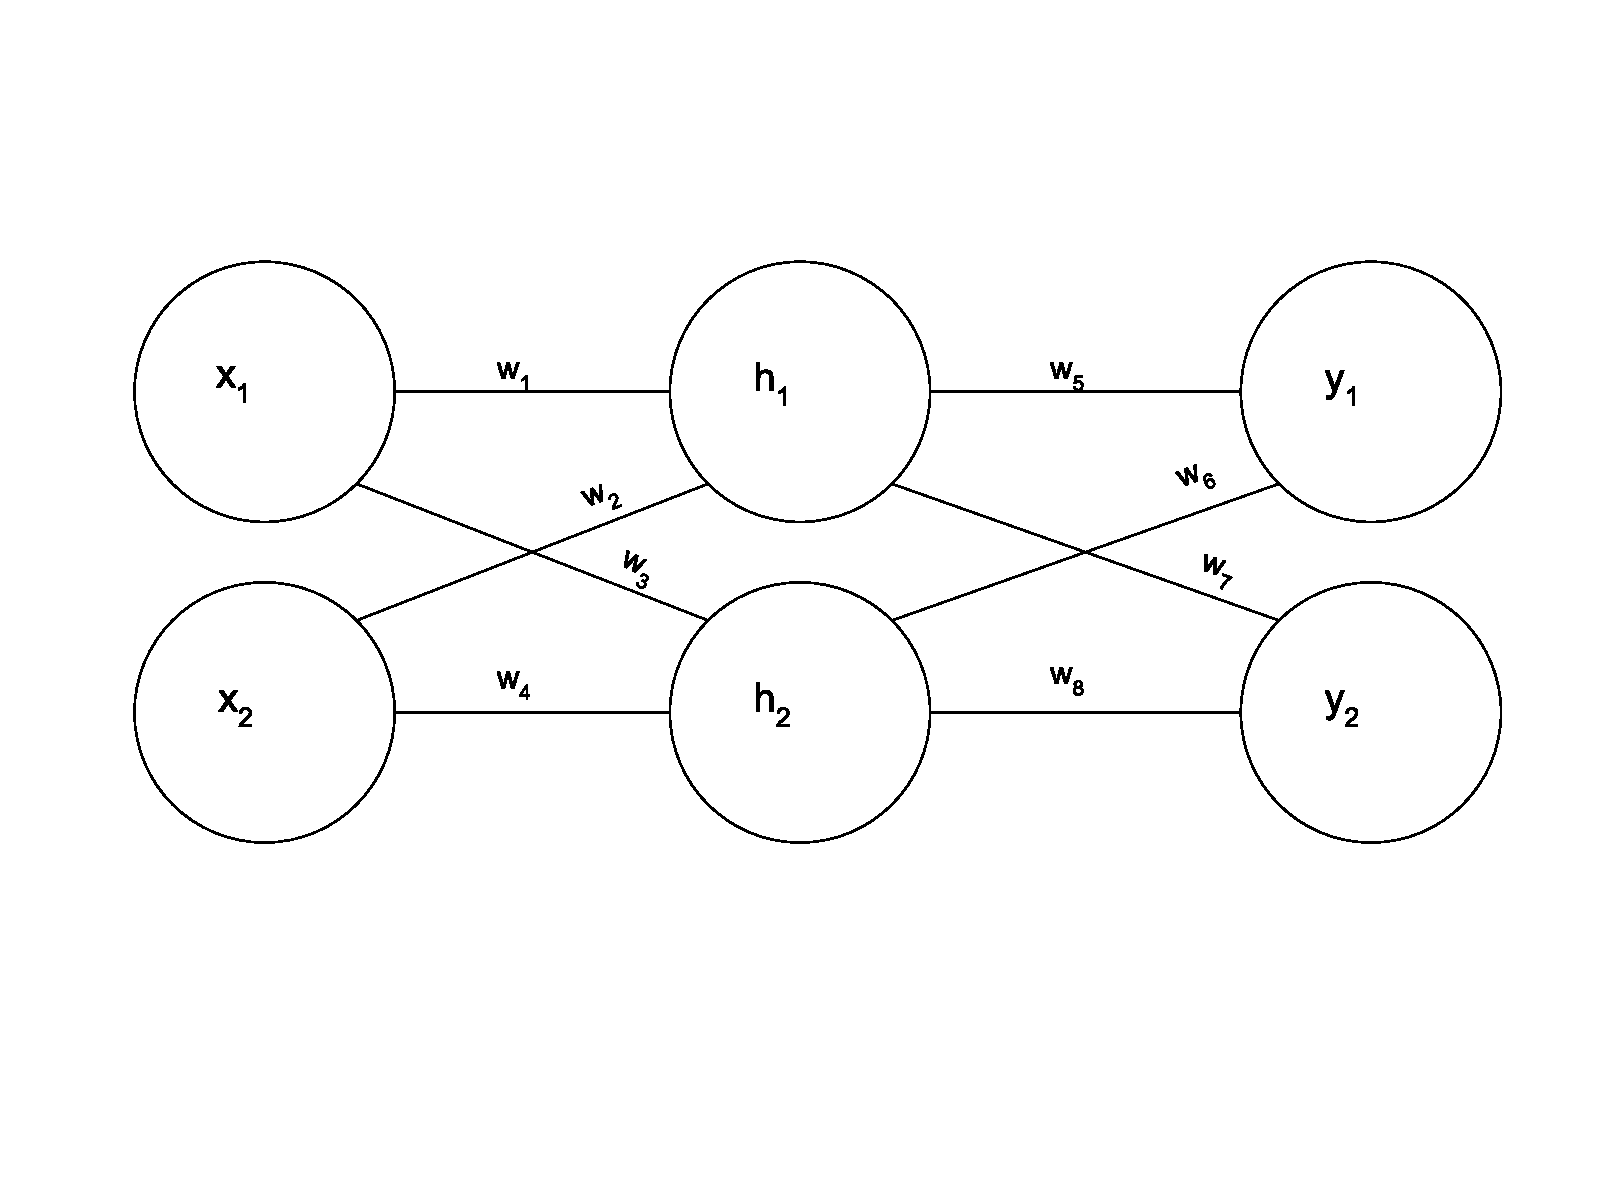
\includegraphics[scale=0.5,trim={0 3cm 0 3cm},clip]{./Figures/smallNN.pdf}
\end{center}
\caption[Simple, Feedforward Neural Network]{Simple, Feedforward Neural Network. \textit{x} denotes an input layer node, \textit{h} a hidden layer node and \textit{y} an output layer node. \textit{w} denotes a connection from a node to the node in the next layer, from left to right.}
\end{figure}

In the simple, feedforward neural network (Figure 2), there is a single input layer, hidden layer, and output layer. Each hidden and output layer is composed of several nodes with some activation function; in the simplest models, threshold linear units (TLU) are used as the nodes.  To predict the output $y_1$, we first propagate the $x_1$ and $x_2$ input values forward, via the connections from the input layer to the output later, and multiply by the corresponding weight. Therefore, the value incoming to $h_1$ can be represented as $\alpha = x_1*w_1 + x_2*w_2$. The threshold linear unit is so named due to the activation function of the node; instead of a sigmoidal activation function, the value is thresholded via an arbitrary threshold $\theta$, such that 

\[ h_1 = \begin{cases}
	0 & \alpha \leq \theta\\
	1 & \alpha > \theta\\
	\end{cases}
\]

The activation of the TLU is loosely based on the circuitry and behavior of biological neurons, where the incoming connections to an node reflect dendritic connections of a neuron, and the threshold behavior reflects the all-or-nothing nature of an action potential, and corresponding signal propagation (Gurney, 2014, 31; Steels, 2007). However, other activation functions are commonly used, such as the sigmoid function (Gurney, 2014, 35-36) $$y(x) = \frac{1}{1+e^{-x}}$$ We calculate in a similar fashion for $h_2$, using the weights at $w_3$ and $w_4$ (Gurney, 2014, 29-30; Hecht-Nielson, 1989). With the newly calculated values at the hidden layer, we perform the same operations on the values to find the prediction values in the output layer. For example, $y_1 = h_1*w5 + h_2*w_6$, where $h_1$ and $h_2$ are the outputs of the hidden layer. $y_2$ follows a similar calculation, with weights $w_7$ and $w_8$(Gurney, 2014, 29-30; Hecht-Nielson, 1989). \par
Once all output node values are calculated, the forward-pass is complete, and the result is a vector of values in the output neurons. We calculate the error to observe the difference between the output values of our network and the target values we want our network to produce. Since we cannot change our input values, the only values we are able to change in the network are the weights of each connection from the input layer to the hidden layer, and from the hidden layer to the output layer. Furthermore, we do not want to randomly change the weights until the network produces an output closer to our target. Instead, we want to slightly alter the weights depending on how each weight contributed to the overall error between the output of the network and the target. These calculations are know as the backward-pass, or backpropagation.\par
Backpropagation shifts the network along the gradient towards convergence of the error and weights. In the presentation of gradient descent presented earlier, we arrived at the definition as an iterative process of the function $$\Delta x_i = -\alpha(\frac{\partial y}{\partial x_i})$$ (Gurney, 2014, 82-85). However, we now apply the function as a minimization process of the \textit{error}, with respect to the \textit{weights} of the neural network. Therefore, the change in weight during a backpropagation step can be represented as $$\Delta w_{ij}= -\alpha(\frac{\partial E}{\partial w_{ij}})$$. The target function to minimize is now the cost function, and the variables to be changed are all weights in the neural network. At the backpropagation step for updating the weights between the output layer and the prior hidden layer in our example simple feedforward neural network, the chain rule is applied on $\frac{\partial E}{\partial w_{ij}} $, which expands to $$\frac{\partial E}{\partial w_{ij}} = \frac{\partial E}{\partial y_j} * \frac{\partial y_j}{\partial I_{j}} * \frac{\partial I_{j}}{\partial w_{ij}}$$ where $i$ denotes the source node, $j$ the target node. The function for finding the change in error with respect to (w.r.t) a change in particular weights is expanded to three calculations: the change in error w.r.t. change in the output of the activation function, the change in the output of the activation w.r.t change in the inputs to the activation function, and the change in the inputs of the activation w.r.t. change in $w_{ij}$ (Gurney, 2004, 89-91; Hecht-Nielson, 1989). The value these calculations evaluate to depends on the error calculation method, the activation function, and how the inputs to the calculation function are calculated; using a TLU in place of a sigmoid function will result in a different $\Delta w_{ij}$.\par
Backpropagation between the hidden and input layers of the follow a similar approach, with a difference in the calculation of error; since we are now calculating for a hidden node, with forward connections to output nodes in the output layer, each hidden neuron contributes to the error contribution of several output nodes. Therefore, we must sum the error contribution over all nodes that the the hidden node contributes to, resulting in $$\frac{\partial E}{\partial w_{ij}} = \sum_{k=I_i}{\frac{\partial E_k}{\partial y_j}} * \frac{\partial y_j}{\partial I_{j}} * \frac{\partial I_{j}}{\partial w_{ij}}$$ where $I_i$ is the set of all neurons in the next forward layer that receive input from the hidden node $k$ that we are backpropagating from (Gurney, 2004, p.100-101; Hecht-Nielson, 1989). Both methods are applied during backpropagation of a neural network, depending on the weight being updated. $\frac{\partial E}{\partial w_{ij}}$ is calculated for all $w_{ij}$ between the output and hidden layers, for every training step, typically until error converges and does not minimize further, successfully performing gradient descent on the error.\par

\subsection{NEST: Generating Training Data}
There are several reasons for generating simulated calcium imaging data for the purposes of network reconstruction. First, generation of simulated calcium imaging data allows for benchmarking of the reconstruction methods employed. In typical calcium imaging data, the ground truth is not known, resulting in a lack of comparison between the reconstructed network and the network targeted for reconstruction. By generating simulated networks and recreating calcium imaging data, we ensure access to the ground truth for comparison with the model. Simulation of training data also permits programming of particular characteristics to the network, and observing the changes of this reconstruction in both the simulated data and the reconstruction of these networks.\par
Machine learning methods are typically trained on some prior data set. Simulation of calcium imaging data provides an easily accessible method of generating data for training and testing the machine learning based model, due to unconstrained and unrestricted access to data, before allowing the model to analyze recorded data that would be ideally used as testing data. Additionally, including a training set ensures that the algorithm is able to remain generalized; that is, the algorithm does not learn to represent that single data set exceptionally well, and fail when a different pattern is presented to the algorithm.\par
The simulations presented here are performed in NEST simulator, a tool maintained by the NEST initiative (Kunkel et al., 2017). The NEST simulator was selected for the purpose of simulations that maintain biological realism and complexity, with emphasis on simulation of large neuronal networks. The advantage NEST has over other simulators is the capability to simulate large networks with varying facets, such as synapse and neuron types, while retaining accurate representation of the individual neurons (Brette et al., 2007).\par
\newpage
\section{Methods}

\begin{figure}[H]
\centering
	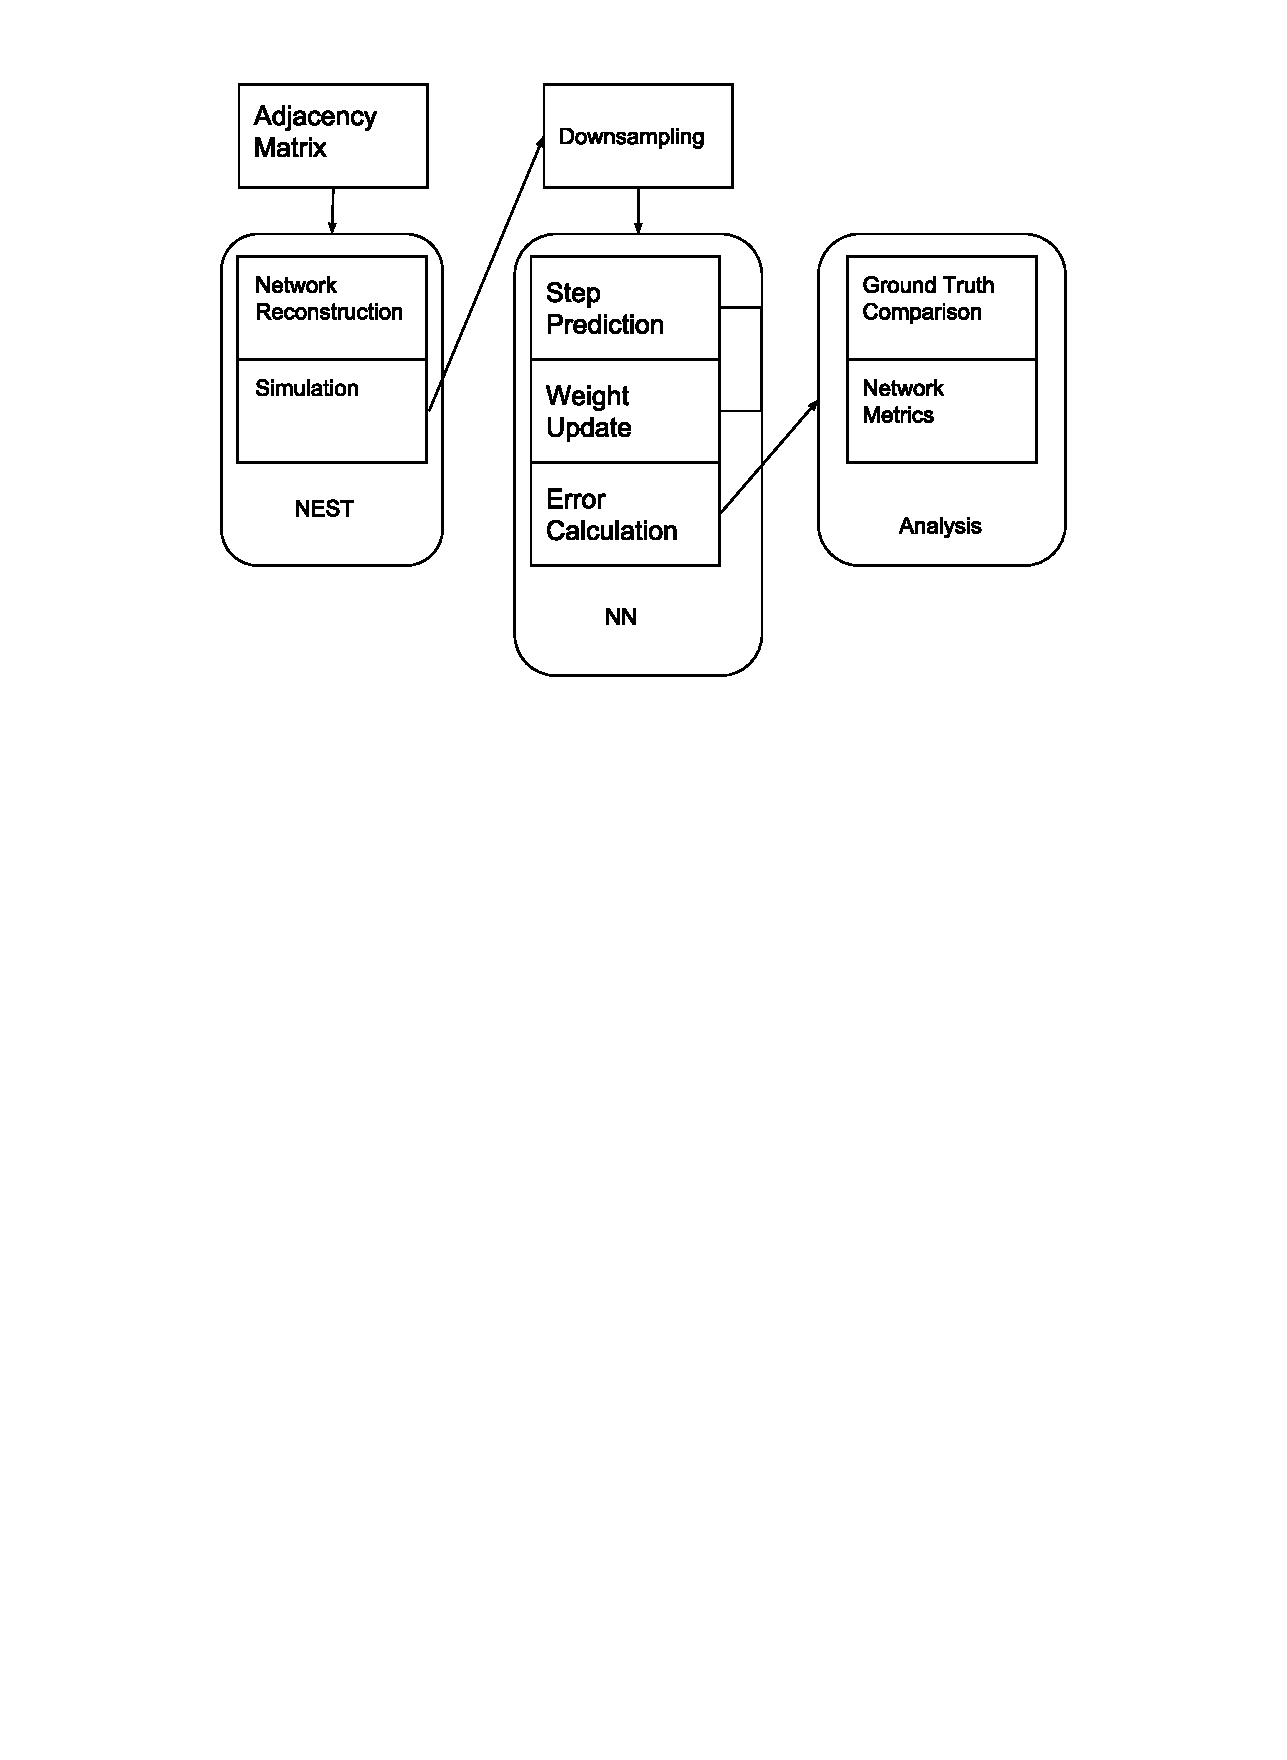
\includegraphics[scale=0.7,trim = {0 18cm 0 1cm},clip]{./Figures/SPROJModel.pdf}
	\caption[Experimental Pipeline]{Experimental Pipeline. We start with a pre-generated adjacency matrix detailing the connections of a population of neurons, and pass it to the NEST simulator program. The NEST simulator reconstructs the network defined by the matrix; at this stage, Poisson noise is added to the population via a connection from a 'noise generator' NEST object to all neurons in the population. The simulation is then run for 10000 time steps (milliseconds), and the generated data is output as a spike time matrix of n x t dimensionality, n = population size and t = time steps. The output is then downsampled to reflect realistic calcium imaging frame duration of 10 ms, reducing the data set to t = time steps/10.}
\end{figure}

\subsection{Random Network Generation}
To generate simulated data, we first create a random network. All random networks here are generated by iterating over a matrix of size $N$ x $N$, where $N$ is the population size. Each entry in the matrix represents a connection from neuron $i$ to neuron $j$, similar to Figure \ref{adjMatrix}, where $i$ is the row and $j$ the column of the matrix. We iterate across all connections that are not self-connections, assigning a 1 or a 0 to indicate a connection or no connection, according to a discrete uniform distribution. Therefore, in connections that are not self-connections, the the likelihood for a connection and for no connection is equal. All self-connections, which are values along the diagonal of the matrix, and where $i$ = $j$, the value is set to 0 to represent no self-connections. Since the number of self-connections in a matrix is equal to the population size, $\frac{1}{N}$ connections are predetermined to be 0, and $\frac{N-1}{N}$ connections are randomly selected across the matrix.\par
Analysis the performance of our models on data simulated from a random network allows us to observe whether degree distribution data is preserved in the simulated spike trains, and the capability of our models to reproduce the degree distributions of the original spike trains from the spike time data.\par

\subsection{Simulation of Neurons for Spike Train Generation}
The NEST simulator is used for the purposes of generating spike train data. NEST Izhikevich neurons are used as the model neurons, due to the increased complexity over leaky integrate-and-fire neurons, and the reduced computational complexity over models of significantly more numerous compartment models, such as the Hodgkin-Huxley models (Brette, 2015; Izhikevich, 2004). NEST implementation dynamics of Izchikevich neurons are provided by the following:

$$dv/dt=0.04v^2+5v+140-u+I$$
$$du/dt=a(bv-u)$$
\smallskip

{\centering
if $v >= V_{th}:\{$\\
$v = c$\\
$u = u + d\}$\par
}
where $v$ represents the membrane potential of the neuron and $u$ the membrane recovery variable. The membrane recovery variable captures the responses of $K^{+}$ and $Na^{+}$, and is a source of negative feedback to $v$. Coefficients for change in membrane potential, are based on scale, with membrane potential at $mV$ and time as ms, as are $a$ and $b$. $I$ is the input current to the neuron, and $c$ and $d$ are the post-spike reset values of the neuron (Kunkel et al., 2017, Izhikevich, 2004). 

To simulate a population of neurons with $n$ population size over $t$ time, a file containing an $n$ x $n$ adjacency matrix is provided to the simulation program, which then creates a NEST neuron population with the exact number of neurons and connections between the neurons in the population, using the corresponding weight of the connection stored in the adjacency matrix. All connections are excitatory connections. Interactions with neurons in NEST must be achieved through the creation of new node objects, made to represent and achieve the results of physical instruments and devices; therefore, we create a Poisson generator node to add noise to the population, and connect a spike detector node to record all spikes in the population during simulation. The population is then recorded over 10000 simulation steps, or 10000 ms. The corresponding output of the simulation is converted to a matrix of $n$ x $t$ dimensionality. The simulation is repeated to produce 100 spike trains from one adjacency matrix.\par
Post-simulation, all data is downsampled from 10,000 ms to 1,000 ms, corresponding to the 10 ms frame rate of calcium imaging. Downsampling is performed by observing consecutive reading frames of size 10 time steps (ms), and checking for occurrences of spikes within the 10 frames. If one or more spikes occur within the frame for a particular neuron, a single spike is recorded for the neuron; otherwise, no spikes are recorded for the neuron. The downsampling produces a dataset that resembles a similar time step size of 10 ms to the \textit{in-vivo} {Xenopus Laevis} calcium imaging data available.

\begin{figure}[H]
\centering
	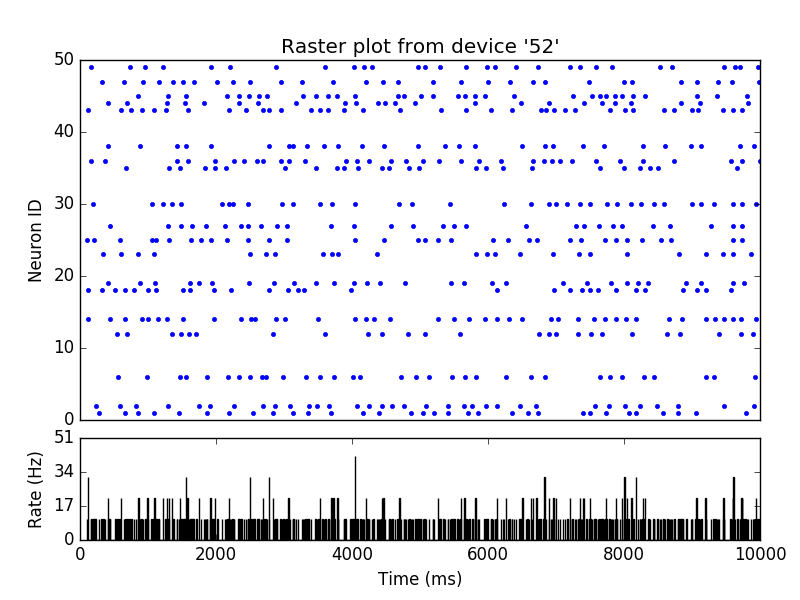
\includegraphics[scale=0.5]{./Figures/figure_1.png} 
	\caption[Raster Plot via NEST Simulator.]{Raster Plot via NEST Simulator. The plot is generated by simulating a population of 50 neurons over 10000 time steps (ms), and graphically represents two distinct arrays output by the simulation: one array consisting of neuron IDs in the population, and another array with the corresponding spike times of the spiking neurons stored in the indices of the former array. The NEST simulator connects each neuron based on the input adjacency matrix and attaches additional noise and spike detection objects to every neuron in the population. Device 52 is the NEST spike detection object; all neurons are connected by the NEST simulation program for the purposes of spike detection. Device 51 is the noise generator object, and Devices 1-50 are the neurons in the population. }
\end{figure}

%\subsection{Page Rank}
%The Page Rank-based algorithm takes a weighted adjacency matrix as an input; a non-weighted adjacency matrix would result in no change in the Page Ranks of each neuron, and no change in the resulting adjacency matrix. The Page Rank for each neuron is then calculated based on the following formula:

%$$PR_i = (1-d)+d(\sum(\frac{PR_j}{C} * W_ij))$$

%Where PR is the Page Rank of neuron $i$, $d$ is the standard damping factor of 0.8, $PR_j$ is the Page Rank of incoming neuron j, and $W_{ji}$ is the weight of the connection from neuron j to i. The summation calculates for all incoming connections to neuron i. The formula is recalculated until convergence, where the Page Ranks no longer change, at which point the weights are updated such that the weight of each connection is multiplied by the Page Rank of the source of the connection. The network is then pruned by comparing the weights between neuron i and j, or Wij and Wji, and the the lower value is reduced to 0, while the higher value is set to 1, preserving the higher connection. The process is then repeated, using the new weights, for an arbitrary number of times.\par

\subsection{Machine Learning Model}\label{ssec:MLM}
\subsubsection{Base Model}\label{sssec:BM}
The supervised learning model presented contains only two layers: an input layer and a hidden layer. We attempt to restrict the number of layers to a single layer, in order to extract a single set of weights that can be understood as the adjacency matrix reflecting the population of neurons from which the spike-train originates. The base model is a two-layer network with the squared error of the form $$E_{total} = \sum{\frac{1}{2}(target-prediction)^2}$$ as the error function, where the target is the $y$ label to a corresponding $x$ input, and prediction is the output of the model after one prediction step (Werbos, 1990; Gurney, 2004, p.86-66; Bohte et al., 2002). The base model has a simple structure of $n$ x 1 dimensionality in each layer, with 2 layers and $n$ x $n$ weights connecting them.\par
First, a single time step is provided from an $t$ x $n$ dimensional matrix, where $t$ is the number of time steps, as an $1$ x $n$ array, where each $n$ is a neuron id corresponding to a specific neuron in the population. The time step is matrix multiplied by the weight matrix of $n$ x $n$, resulting in the prediction array of $1$ x $n$. Each value in the prediction array is passed to the sigmoid activation function $$ f(x) = \frac{1}{1 + e^{-x}}$$ and updated as the prediction of the active and inactive neurons in the next time step. Therefore, the backpropagation step calculates the weight changes $$\frac{\partial E}{\partial w_{ij}} = \frac{\partial E}{\partial y_j} \cdot \frac{\partial y_j}{\partial I_{j}} \cdot \frac{\partial I_{j}}{\partial w_{ij}}$$ where the partial derivative of the error w.r.t the prediction $y_j$ and target $\hat{y_j}$ expands to $$\frac{\partial E}{\partial y_j} = -(\hat{y_j} - y_j) $$ due to the summation in the error function; all other predictions are held constant, which results in a zero derivative for the remainder of the summation outside of $y_j$. The partial derivative of the output of the activation function $y_j$ w.r.t. the input $I_j$, or the results of the first matrix multiplication, evaluates to $$\frac{\partial y_j}{\partial I_j} = \frac{e^{I_j}}{(1+e^{I_j})^2} = y_j \cdot (1 - y_j)$$ Finally, the partial derivative of the input to the activation function $I_j$ w.r.t. the weight being updated $w_{ij}$ is $$\frac{\partial I_j}{\partial w_{ij}} = 1 \cdot x_i \cdot w_{ij}^{1-1} = x_i$$ Therefore, the full learning rule applied in this model is $$ \frac{\partial E}{\partial w_{ij}} = -(\hat{y_j}-y_j) \cdot (y_j \cdot (1-y_j))\cdot x_i$$ At every time step, the learning rule is applied to the current input and predicted next time step, and each traversal across the entire dataset is an iteration of the learning process.\par
\bigskip
\bigskip
\bigskip
\begin{algorithm}[H]
	\caption{Base Model}
	Initialize the weight matrix of $n$ x $n$ size with random values 0-1.\\
	Initialize dataset as spike-time matrix\\
	i = A time step in the spike-time matrix\\
	\For {i $<$ {\normalfont number of spike Times}}{
		Calculate dataset[i]*weights $\rightarrow$ outputs (1 x $n$)\\
		Multiply each value in outputs by the activation function\\
		return the 1 x $n$ dimensional array of predictions of activity in the next time step\\
		$j$ = index of the source neuron in the weight matrix\\
		$k$ = index of the target neuron in the weight matrix\\
		$w_{jk}$ = a weight in the weight matrix corresponding to indices j,k\\
		\For {$w_{jk}$ {\normalfont in the weight matrix}}{
			Calculate $\Delta w_{jk} = \frac{\partial E}{\partial w_{jk}}$\\
			Update the weight via $w_{jk} = w_{jk} -\alpha(\Delta w_{jk})$
			}
		}
	Generate a new set of predictions P' with the calculated Matrix\\
	Calculate the mean squared error between P'[0:length-1] and dataset[1:length]
\end{algorithm}
\clearpage
\subsubsection{Variable Activation Function Model}\label{sssec:VAF}
The variable activation function model contains two additional sets of values in two separate $n$ x 1 dimensional arrays, where $n$ is the size of the population of observed neurons. Each value in the matrix corresponds to a particular node in the output layer of the same index. Therefore, the activation function is modified to a general logistic function of the form $$ f(x) = \frac{1}{1+e^{-a(x - b)}}$$ where $a_j$ and $b_j$ are the values corresponding to the unique steepness, or shape, and center, defined as the value at which the second derivative of the function changes signs, of the activation function for target output node $y_j$, allowing for a distinct activation function for each output node. The error is backpropagated in a similar fashion to the weights between the input and output layers of the model, and simultaneous to the weight updating step. To update the steepness of the of output $y_j$, we calculate $\Delta a_j$ as
 $$\Delta a_j = \frac{\partial E}{\partial a_j} = \frac{\partial E}{\partial y_j} \cdot \frac{\partial y_j}{\partial a_j}$$
 where $\frac{\partial E}{\partial y_j}$ is evaluated as in the base model, and the partial derivative of the output $y_j$ w.r.t logistic function steepness $a_j$, $\frac{\partial y_j}{\partial a_j}$, is 
 $$\frac{\partial y_j}{\partial a_j}=\frac{e^{-a_j(x-b_j)}(b_j - x)}{(1+e^{-a_j(x-b_j)})^2}$$, where $x$ is the input to the activation function. The change of the logistic function center at the update step is given by 
 $$\Delta b_j = \frac{\partial E}{\partial b_j} = \frac{\partial E}{\partial y_j} \cdot \frac{\partial y_j}{\partial a_j}$$ 
 where the partial derivative of the output $y_j$ w.r.t logistic function center $b_j$, $\frac{\partial y_j}{\partial b_j}$ is calculated as 
 $$\frac{\partial y_j}{\partial b_j} = \frac{a_je^{-a_j(x - b_j)}}{(1 + e^{-a_j(x - b_j)})^2} $$

The inspiration for this variable activation function model is primarily based on biological neuronal activation, the postsynaptic potential. As discussed in section \ref{ssec:Neuron}, postsynaptic potential occurs upon binding of neurotransmitters released from the presynaptic neuron to receptors in the postsynaptic neuron. However, synapses are dynamic; synaptic potentiation, augmentation, facilitation,  and depression can occur, and are dependent on the timing and magnitude of neurotransmitter binding to the postsynaptic neuron (Purves, 2004, 582; Zucker, 1989). Synaptic potentiation, augmentation, and facilitation are forms of increase in synaptic strength, where the postsynaptic potential is greatly increased compared to an isolated postsynaptic potential (Zucker, 1989; Purves, 2004, 582). These forms of synaptic plasticity are differentiated primarily by the duration of strengthening (Zucker, 1989; Purves, 2004). Contrastingly, synaptic depression is weakening of the synaptic strength, and can vary in duration (Zucker, 1989; Purves 2004, 582). These possible changes to the synapse result in neurons that differ in requisite magnitude of neurotransmitter binding for a postsynaptic event. In artificial neural network terminology, nodes have distinct thresholds for activation, and distinct activation functions. Therefore, this novel implementation of the model with a variable activation function may capture dynamics not described in the underlying weight matrix of the model.\par
\bigskip
\bigskip
\bigskip
\begin{algorithm}[H]
	\caption{Variable Activation Function Model}
	Initialize the weight matrix of $n$ x $n$ size with random values 0-1.\\
	Initialize dataset as spike-time matrix\\
	i = A time step in the spike-time matrix\\
	\For {i $<$ {\normalfont number of spike Times}}{
		Calculate dataset[i]*weights $\rightarrow$ outputs (1 x $n$)\\
		Multiply each value in outputs by the activation function\\
		return the 1 x $n$ dimensional array of predictions of activity in the next time step\\
		$j$ = index of the source neuron in the weight matrix\\
		$k$ = index of the target neuron in the weight matrix\\
		$w_{jk}$ = a weight in the weight matrix corresponding to indices j,k\\
		\For {$w_{jk}$ {\normalfont in the weight matrix}}{
			Calculate $\Delta w_{jk} = \frac{\partial E}{\partial w_{jk}}$\\
			Update the weight via $w_{jk} = w_{jk} -\alpha(\Delta w_{jk})$\\
			}
		\For {$a_j$ {in the steepness matrix}}{
			Calculate $\Delta a_j = \frac{\partial E}{\partial a_j}$, $\Delta b_j = \frac{\partial E}{\partial b_j}$\\
			Update the steepness and center via $a_j = a_j -\alpha(\Delta a_j)$, $b_j = b_j -\alpha(\Delta b_j)$
			}
		}
	Generate a new set of predictions P' with the calculated Matrix\\
	Calculate the mean squared error between P'[0:length-1] and dataset[1:length]
\end{algorithm}
\clearpage
\subsection{Cross-Correlation}
We compare the performance of the model to the cross-correlation method of inferring connectivity. Cross-correlograms here are produced using the \textit{elephant} and \textit{neo} python packages; these packages assist in calculating the cross-correlation matrix by producing cross-correlograms for the input spike trains. The cross-correlogram method of extracting spike-train correlations compares the spike times of a reference train to a target train. Different time steps within a defined window are observed in the target train, using a spike in the reference train as the origin. For each spike in the reference spike train, the spikes in the target spike train are counted in the bins according to the time lag, where the origin time 0 is set to the time of the reference spike in the reference spike train. The final cross-correlation analysis compares over 100 distinct simulated spike time datasets across a population of 10 neurons, with window size [-10,10], as displayed in Figure \ref{main:f}.\par
To designate the highest probability of connections in spike trains from a spike time matrix, we calculate the cross-correlogram for each combination of spike train in the spike time matrix, and find the time bin with the largest amount of counts. This count value is calculated for all combinations of neurons in the spike time matrix, and normalize the values between 0 and 1. Since auto-correlograms represent self-connections and contain the highest counts, where each auto-correlogram max value is equivalent to the number of spikes occuring in the spike train of the neuron, we ignore the auto-correlograms when normalizing the adjacency matrix.

\begin{figure}[H]
\begin{minipage}{.49\linewidth}
\captionsetup{position=top}
\centering
\subfloat[]{\label{main:a}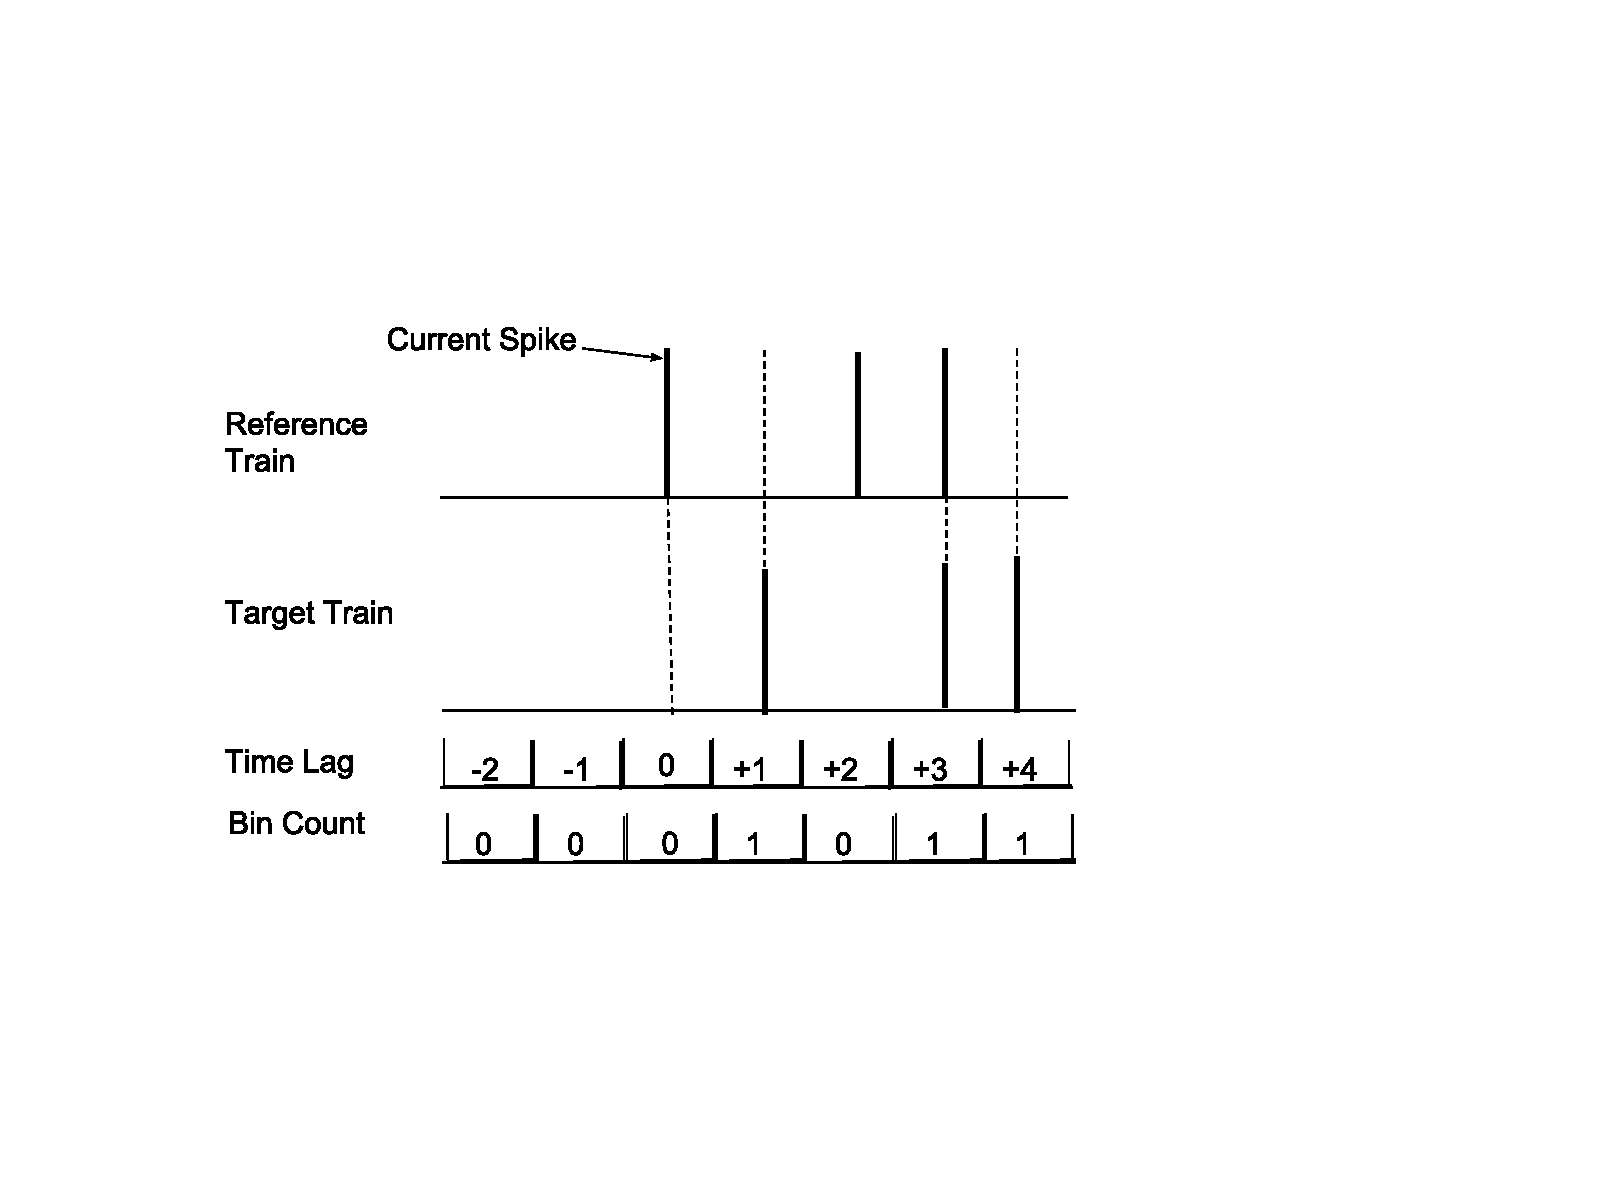
\includegraphics[height=5cm,scale=0.5,trim={3cm 4.5cm 9cm 3cm},clip]{./Figures/"XC Figures"/xcEx.pdf}}
\end{minipage}
\begin{minipage}{.5\linewidth}
\captionsetup{position=top}
\centering
\subfloat[]{\label{main:b}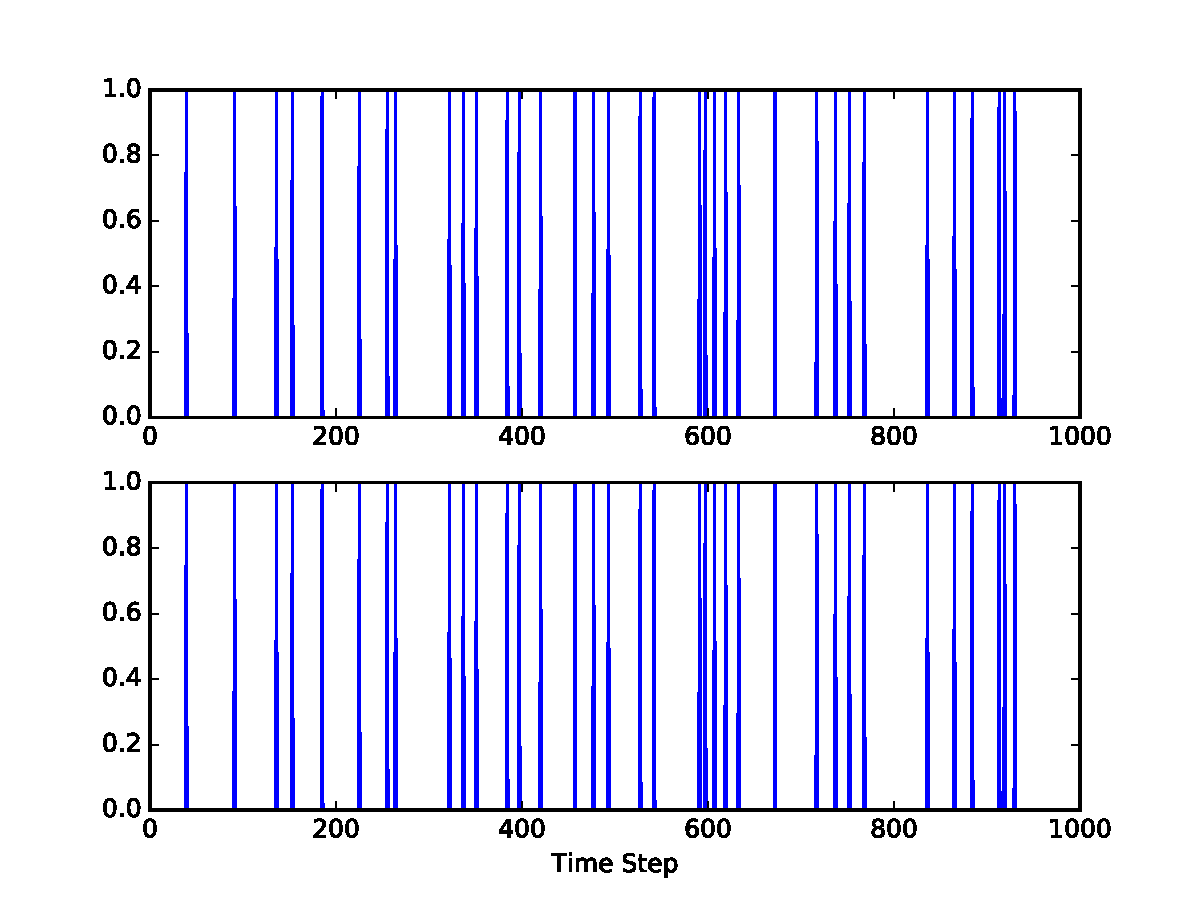
\includegraphics[height=5cm,scale=0.4,trim={1cm 0.5cm 1cm 0},clip]{./Figures/"XC Figures"/AutoCorr.pdf}}
\end{minipage}
\begin{minipage}{.49\linewidth}
\captionsetup{position=top}
\centering
\subfloat[]{\label{main:c}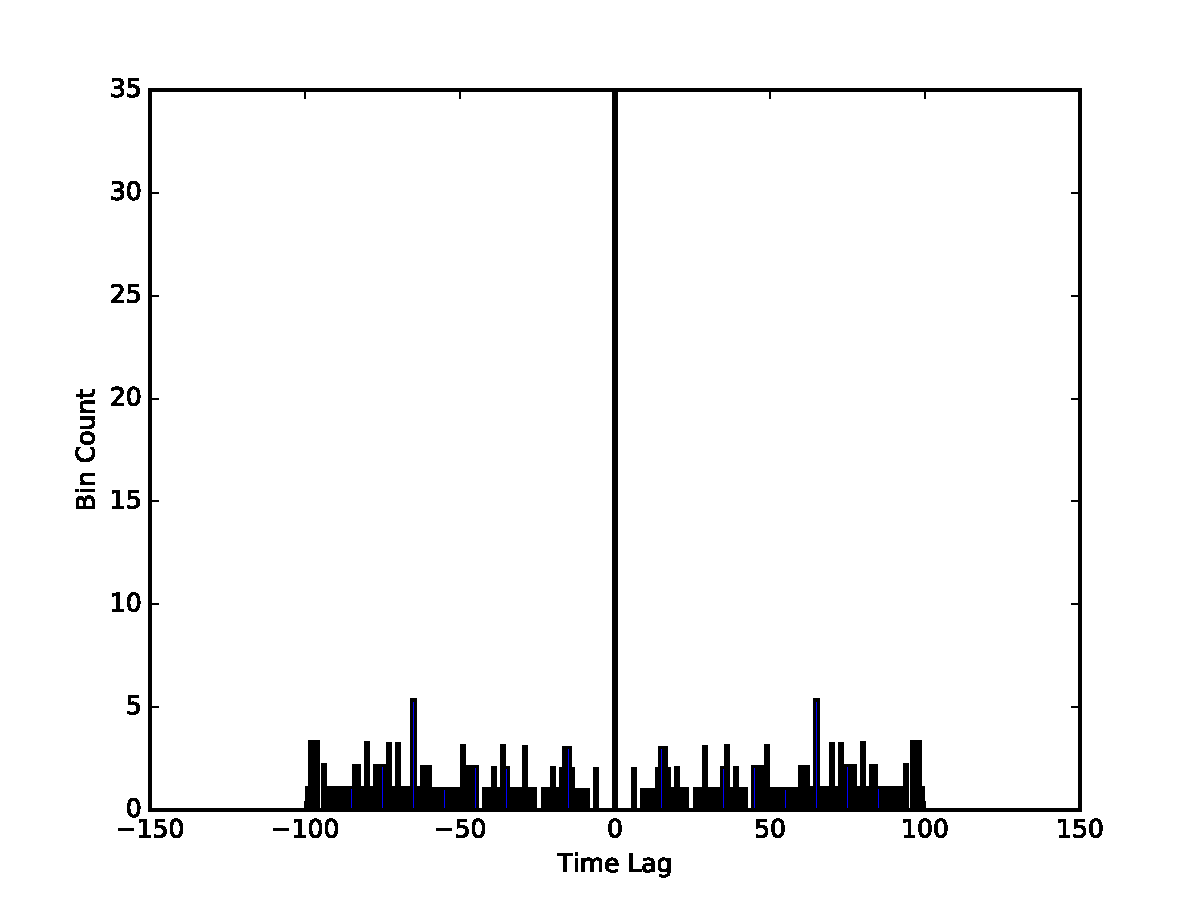
\includegraphics[height=5cm,scale = 0.4,trim={1cm 1cm 1cm 1cm},clip]{./Figures/"XC Figures"/AutoCorrGram.pdf}}
\end{minipage}
\begin{minipage}{.5\linewidth}
\captionsetup{position=top}
\centering
\subfloat[]{\label{main:d}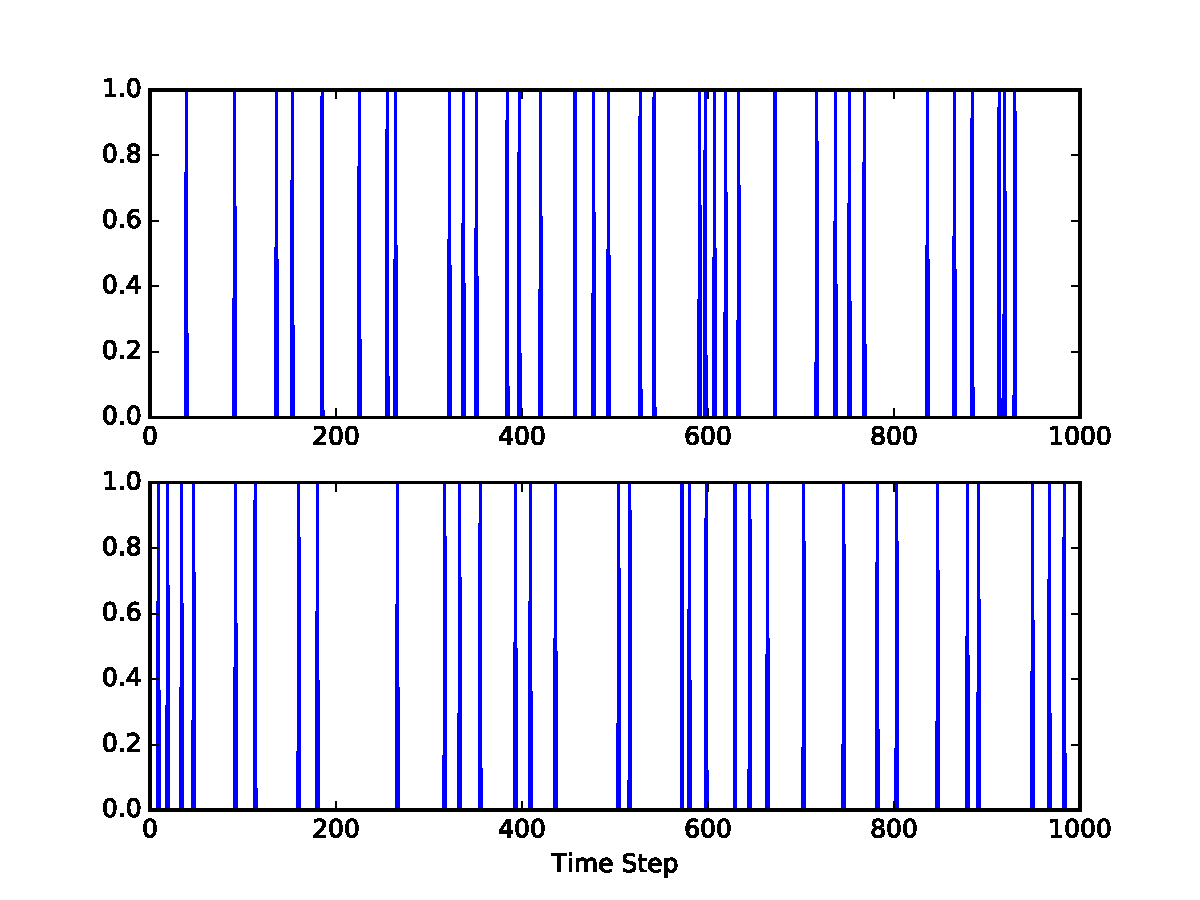
\includegraphics[height=5cm,scale=0.4,trim={1cm 0.5cm 1cm 0},clip]{./Figures/"XC Figures"/05Corr.pdf}}
\end{minipage}
\begin{minipage}{.49\linewidth}
\captionsetup{position=top}
\centering
\subfloat[]{\label{main:e}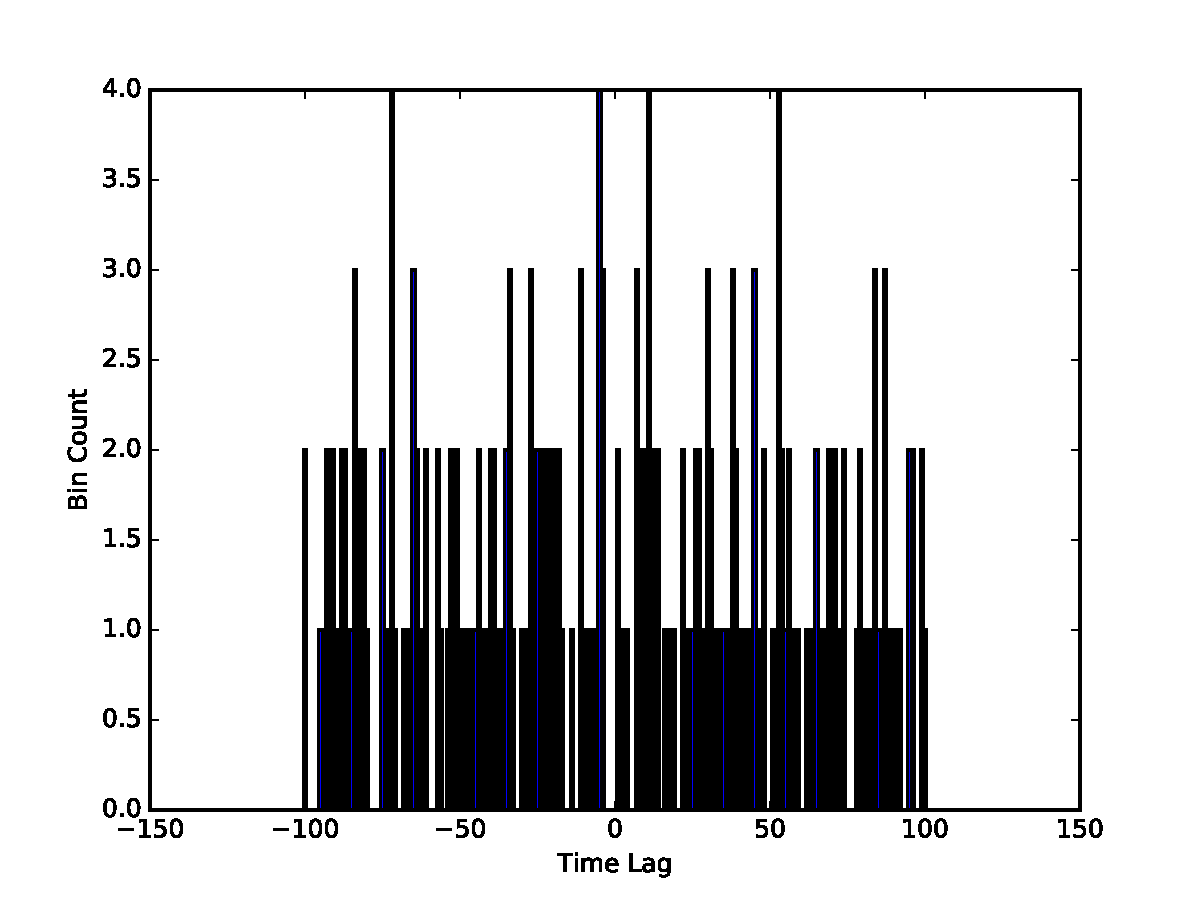
\includegraphics[height=5cm,scale=0.4,trim={1cm 0.4cm 1cm 1cm},clip]{./Figures/"XC Figures"/05CorrGram.pdf}}
\end{minipage}
\begin{minipage}{.5\linewidth}
\captionsetup{position=top}
\centering
\subfloat[]{\label{main:f}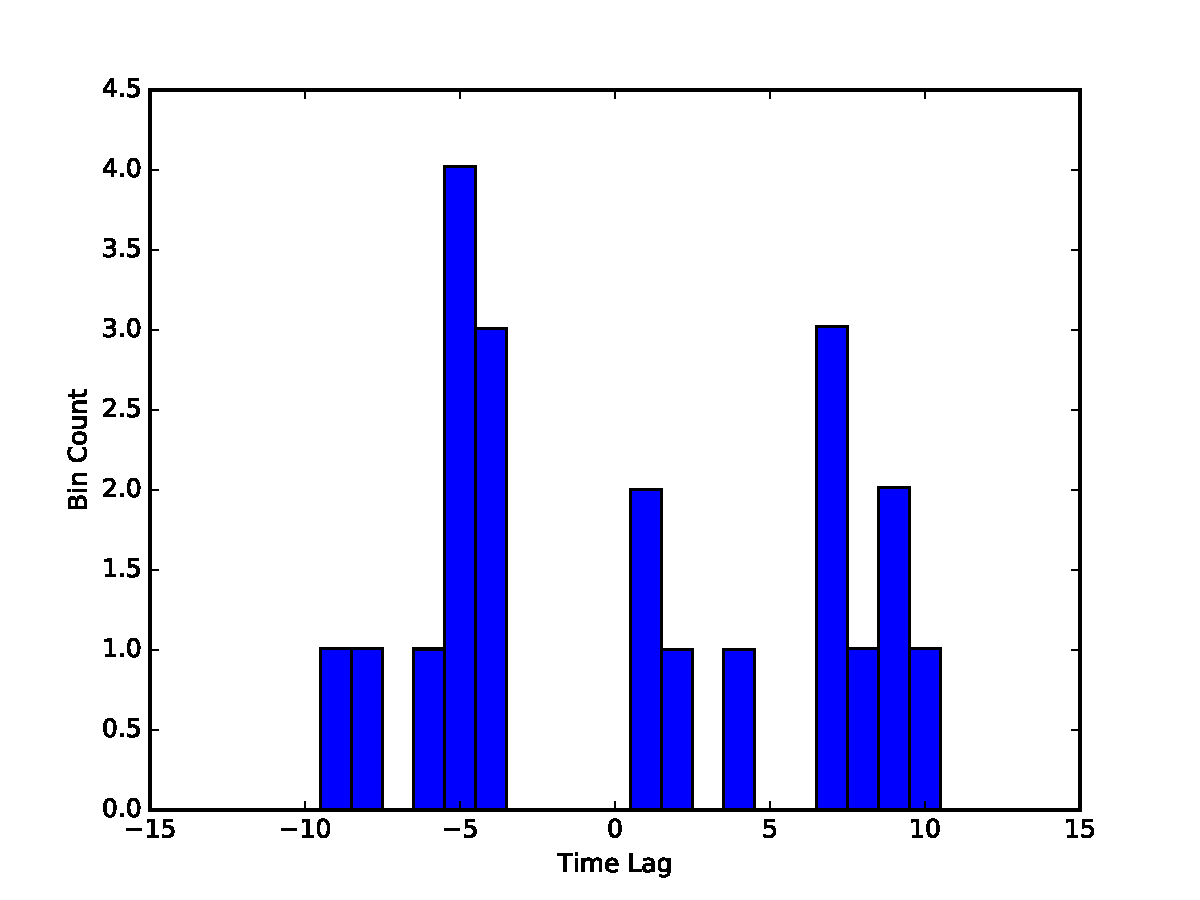
\includegraphics[height=5cm,scale=0.4,trim={1cm 0.4cm 2cm 1cm},clip]{./Figures/"XC Figures"/051CorrGram.pdf}}
\end{minipage}

\caption[Cross-Correlation Histogram (Cross-correlogram) Procedure and Example.]{\textbf{Cross-Correlation Histogram (Cross-correlogram) Procedure and Example.} (a) The cross-correlogram method of relating spike-trains. A spike is selected and designated as the reference point. If a spike appears in the target train at a particular time lag, the value for that bin is incremented.(b)An example autocorrelation spike-train. The top and bottom spike trains are the same spike-train; all spikes align.(c) The autocorrelogram calculated from (b), with a window range of [-100,100]. In an autocorrelation, the highest bin count should be equivalent to the number of spikes in the observed train, and the highest bin is at time lag 0.(d) Two distinct spike-trains. Note the periodic nature of the histogram, identified in (f) (e)Cross-correlogram of (d). (f)Cross-correlogram of (d), window range of [-10,10].}
\label{fig:main}
\end{figure}

\subsection{Xenopus Laevis Calcium Imaging Data}
Calcium imaging data of \textit{Xenopus Laevis} optic tectum activity was provided by Professor Arseny Khakhalin of Bard College. For \textit{in-vivo} recordings, samples were incubated in a diluted OGB1-AM calcium indicator and viewed under a Nikon E600FN 40X objective with a OBG1 filter set. The neurons were illuminated by a high-power blue LED to generate green fluorescence from the calcium indicator, which was projected to the CCD surface of a high-speed neural imaging camera (Xu et al., 2011). The imaging time was 4 s, with 10 ms between each frame. For each recording, approximately 30-80 fluorescent tectal neurons were imaged in the same field of view.\par
Visual stimulation to the tadpoles was administered via a high-fidelity image fiber. Images of varying patterns were projected to one end of the imaging fiber via a miniature LCD screen backlit powerful light emission diode , and the other end was brought to the tadpole's eye (Khakhalin et al. 2014). Three types of visual stimuli were repeatedly displayed to the tadpole's eye in a cyclical manner; first a looming stimulus, then a flash stimulus, and finally a scrambled looming stimulus. Whole flash stimulus is a whole-field illumination, while the looming stimulus is grows from the center of the field towards a whole field illumination, and the scrambled looming randomly selects points of illumination towards a whole field illumination (Jang et al., 2016).\par
After calcium imaging recording, field of interest of approximately 40 pixels were defined around each neuron. Fluorescence within the field of interest were measured over time, and the change in fluorescence activity within a field of interest was calculated by  normalizing the average intensity of the field by an established baseline intensity (Xu et al., 2011). The data is then deconvoluted via the fast non-negative deconvolution algorithm presented in Vogelstein et al., 2010. The resulting deconvoluted calcium imaging trace infers possible spiking for each neuron at each time step.\par
The \textit{Xenopus Laevis} calcium imaging data, after deconvolution, is a spike time matrix with probabilistic values between 0 and 1. These deconvoluted probability values are proportional to the inferred calcium fluorescence increase for a given spike (Vogelstein et al., 2010). To obtain binary values from probability value representations present in the \textit{Xenopus Laevis} calcium imaging data, all non-zero values are denoted as spikes.\par

% Inthe case of the resultant spike time matrices produced by the machine learning models, the matrices are normalized between 0 and 1, and thresholded at 0.5, where values greater than or equal to 0.5 indicate a spike, and values below indicate no spiking. Spike rates from the prediction spike time matrices are inversely calculated in the variable activation function model, where a 0 indicates spiking and 1 indicates no spiking.\par

\clearpage
\subsection{Degree Distribution Calculation}
The \textit{degree} of a node is the number of edges, or connections, to that node (Costa et al., 2005; Hernandez and Miegham, 2011). The degree distribution is a distribution of probabilities. The probabilities are of a node $n$ containing degree $k$ number of connections, and is given by $$Pr[D=k] = \frac{d_k}{N}$$ where $d_k$ denotes the number of nodes with degree $k$ and $N$ is the population size (Hernandez and Miegham, 2011). Indegrees, outdegrees, and total degrees for each node are calculated from adjacency matrices of the population, where the rows indicate an outgoing connection and columns indicating incoming connections. Indegrees are the number of incoming connections to a neuron in a directed network, outdegrees the number of outgoing connections from a neuron, and total degree is the total number of connections to that neuron. The total degree is obtained by adding the indegrees and outdegrees. The total degree distribution, indegree distribution, and outdegree distribution are then calculated for the adjacency matrix.\par
%The spike rate $R$ of neuron $n$ is calculated by $$R_n = \frac{1}{T}\sum_{t=0}^T{s_t} $$where $T$ is the total number of time steps in the spike time matrix, and $s_t$ is the value of time step $t$ for neuron $n$. In practice, the spike rate of a particular neuron $n$ is obtained from the spike time matrix by summing the column, or the activity of neuron $n$ over all time steps in the spike time matrix, and dividing by the total number of time steps in the spike time matrix. Activity is denoted with a 1 the spike time matrix, and no activity denoted with a 0.\par
\newpage
\section{Results}

\subsection{Error}

\subsubsection{Minimum Working Example Convergence}
We first test the model on a miniumum working example to ensure the backpropagation implementations described in sections \ref{sssec:BM} and \ref{sssec:VAF}, and to demonstrate learning and error convergence of the sigmoid function arrays in the variable activation function model described in section \ref{sssec:VAF}. We run the models across two time steps, where a single time step represents 10 ms in the downsampled data, with at least a single observed spike difference between the two steps, to observe the rate of error convergence and capability of the models to predict from a single time step to the next time step. Error is calculated between the prediction of the model and the known target time step using mean squared error of the output. Figure \ref{errorTwoTime:a} and Figure \ref{errorTwoTime:c} demonstrate the subcase of running the model on two time steps and observing the error after each iteration, over 100 iterations, where the two time steps feature a single spike at the input time step and a single spike in the output time step. The other subcases present in the training data were combinations of up to four spikes occurring in any given time step. In the simulated spiking of population size $N$ = 10, across 100 distinct simulations, 73,481 time steps had a spike count of zero, 22,499 contained a single spike, 3568 contained two spikes, 427 contained three spikes, and 25 time steps contained four spikes, indicating 16 possible subcases for the number of spikes in the input and output time steps. However, some subcases, such as two consecutive time steps containing four spikes each, did not appear. The two models each behaved differently when training on different subcases, as indicated by the wide standard deviation bars in Figure \ref{errorTwoTime:b} and Figure \ref{errorTwoTime:d}, where each plot contains information concerning 10 of the 16 possible subcases. These subcases all occurred within the same spike time dataset. The wide standard deviation bars indicate a high variability in the model training error of Figure \ref{errorTwoTime:b} and Figure \ref{errorTwoTime:d}, where 10 different subcase errors are plotted, indicating that performance of both models vary, depending on which time steps the model was being trained on. 

\begin{figure}[H]
\begin{minipage}{0.49\linewidth}
\captionsetup{position=top}
\subfloat[]{\label{errorTwoTime:a}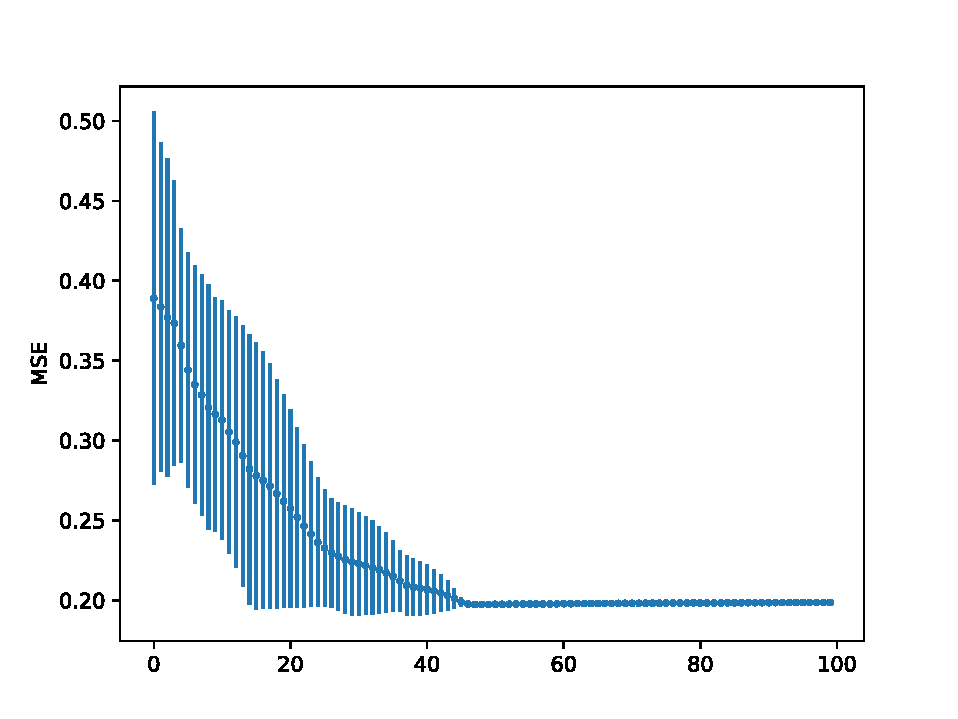
\includegraphics[scale=0.50,trim={0 0 1cm 0},clip]{./Figures/Errors/twoTimeStepVarSigPOPError.pdf}}
\end{minipage}
\begin{minipage}{0.5\linewidth}
\captionsetup{position=top}
\subfloat[]{\label{errorTwoTime:b}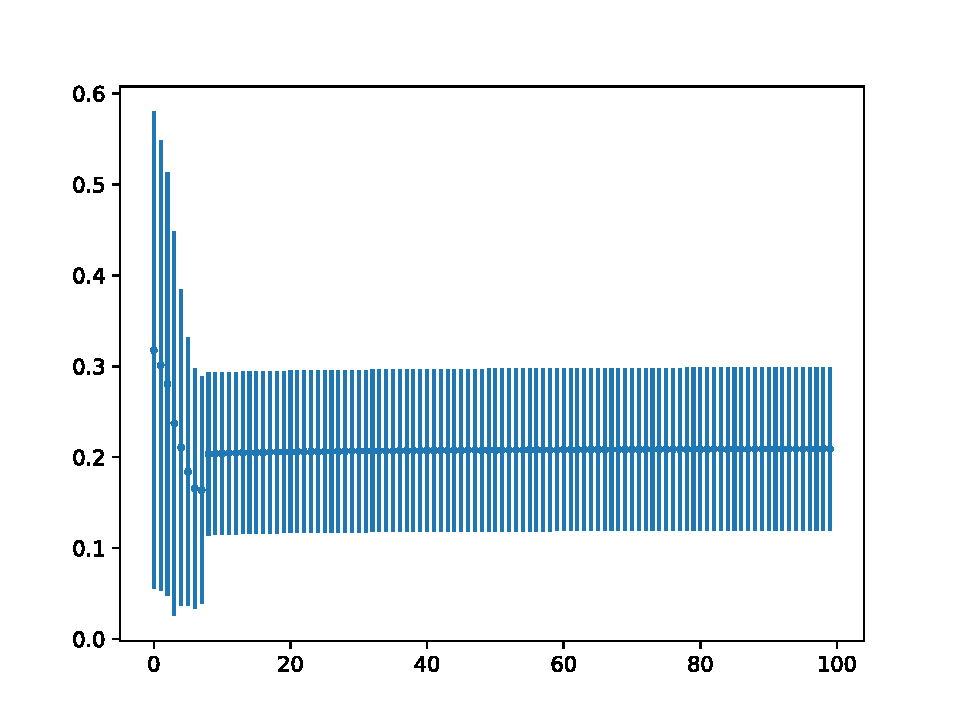
\includegraphics[scale=0.50,trim={1cm 0 1cm 0},clip]{./Figures/Errors/twoTimeVarSigDiffTimesError.pdf}}
\end{minipage}
\begin{minipage}{0.49\linewidth}
\captionsetup{position=top}
\subfloat[]{\label{errorTwoTime:c}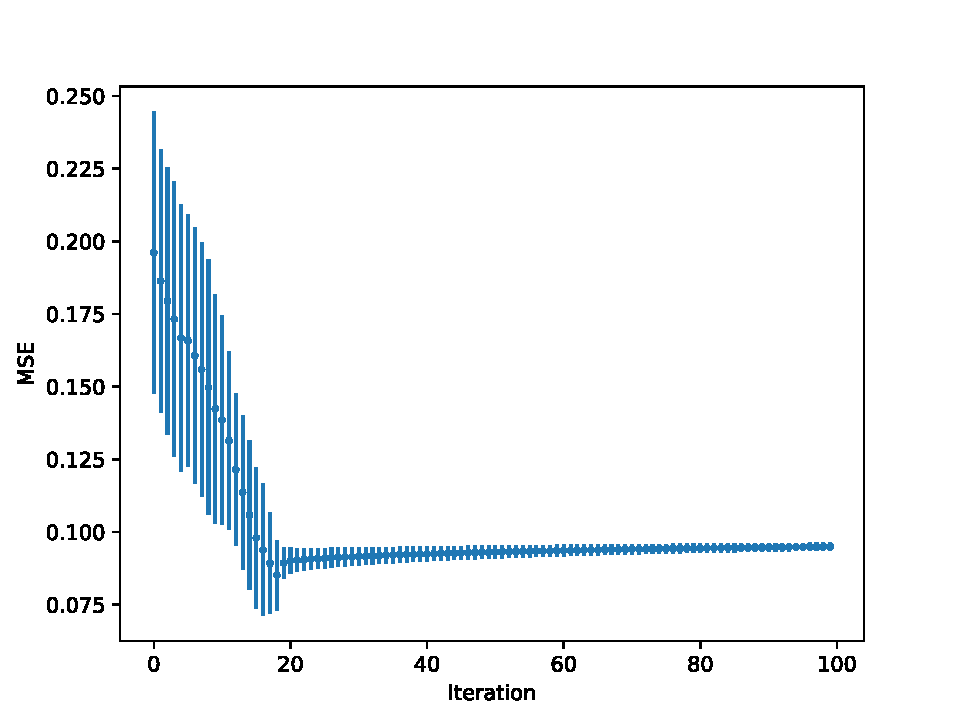
\includegraphics[scale=0.50,trim={0 0 1cm 0},clip]{./Figures/Errors/twoTimeStepCOEPOPError.pdf}}
\end{minipage}
\begin{minipage}{0.5\linewidth}
\captionsetup{position=top}
\subfloat[]{\label{errorTwoTime:d}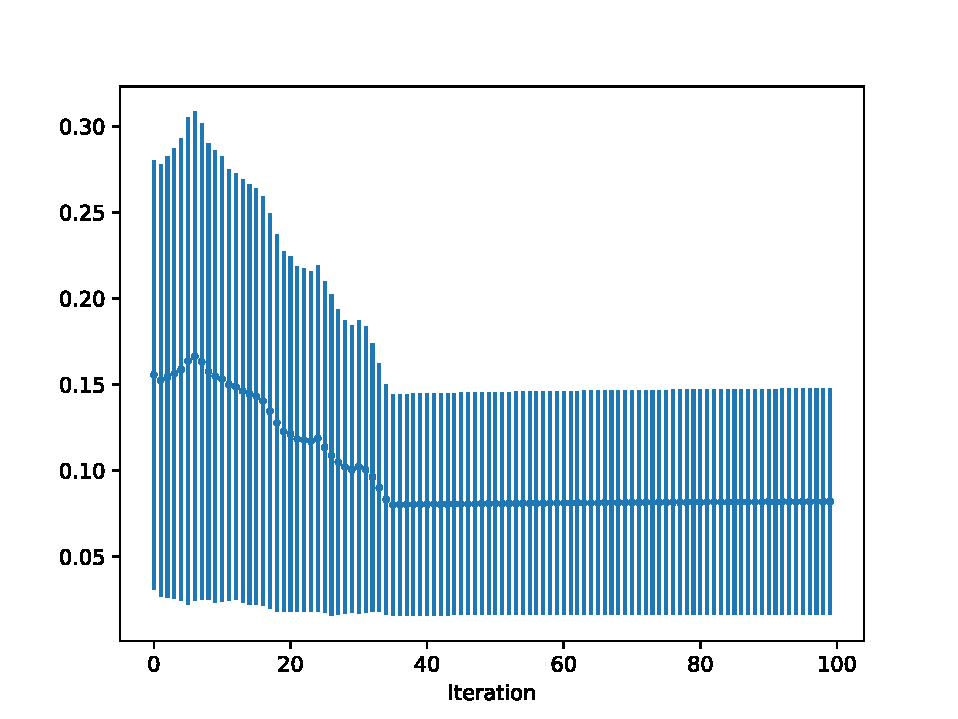
\includegraphics[scale=0.50,trim={1cm 0 1cm 0},clip]{./Figures/Errors/twoTimeStepCOEDiffTimesError.pdf}}
\end{minipage}

%make it clear that a is 1,1 and b takes all of the data
\caption[Error Convergence of Model On Two Consecutive Time Steps.]{\textbf{Error Convergence of Model On Two Consecutive Time Steps.} Each plot represents an average of 10 separate runs of the model, each run lasting 100 iterations. (a)Error Convergence on Variable Activation Function Model. The model was trained on a selected time step, where the first time step contained a single spike, and the following contained a single spike in a different neuron (subcase [1,1]). (b)Average error across ten separate runs of differing subcases with distinct spiking patterns. The subcases are as follows: [0,0], [0,1], [0,2], [0,3], [1,1], [1,2], [2,0], [2,1], [2,2], and [3,0], where the first value is the number of spikes in the input time step, followed by the number of spikes in the output time step. (c) Error calculation using the identical time step to (a), with the base model.(d) Error calculation using the identical distinct time steps to (b), with the base model.}
\label{fig:errorTwoTime}
\end{figure}

%\subsection{Spike Rate Analysis}
%The spike rates of the original spike time matrix inputs to the models are calculated and compared to the spike rates of the predicted activity resulting from the final calculated weights, and, in the case of the variable activation function model, the calculated sigmoid steepness and center arrays.\par
%In the case of the variable activation function model, the spike rates were calculated inversely, where a 0 designates a spike and a 1 designates no spike for a particular neuron at a particular time step,
\clearpage
\subsection{Degree Distribution}
Degree distribution analysis was performed on the final weight matrices produced by the models for both simulated and \textit{Xenopus Laevis} calcium imaging recordings, with a threshold of 0.50, with population sizes of 10 and 50 for the simulated data adjacency matrices; in \textit{Xenopus} calcium imaging data, the population size varied, depending on the recording. The average degree distributions of the predicted adjacency matrices from simulated data are calculated by averaging the degree distribution over all predictions. Calculations of the average degree distribution from the calcium imaging data predictions are performed in the same fashion, over 6 predicted adjacency matrices from 6 \textit{in-vivo} calcium imaging recordings from \textit{Xenopus Laevis}. The average degree distributions differed between the simulation prediction adjacencies (Figures \ref{DD:c} and \ref{DD:d}) and the calcium imaging prediction adjacencies (Figures \ref{DD2:a} and \ref{DD2:b}); where the simulated data produced an average degree distribution resembling a normal distribution, the average degree distribution calculated at the same threshold value of 0.5 from the calcium imaging data resembles a power-law distribution, in both the base model and the variable activation model.

\begin{figure}[H]
\begin{minipage}{0.49\linewidth}
\captionsetup{position=top}
\subfloat[]{\label{DD2:a}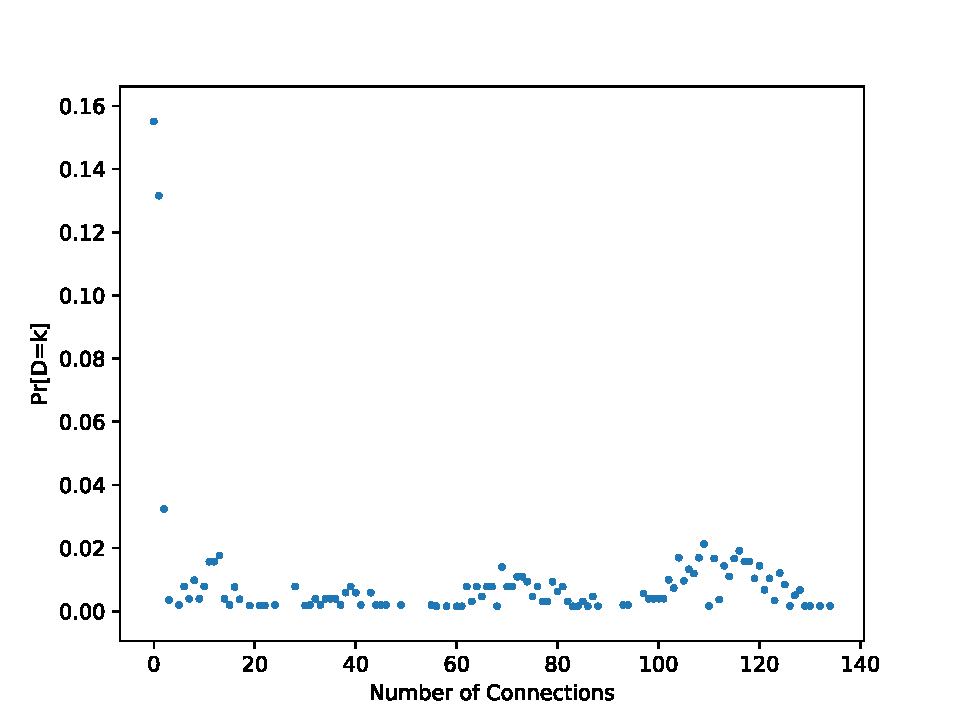
\includegraphics[scale=0.50,trim={0 0 1cm 1cm},clip]{./Figures/DD/caDatavarDDPop50.pdf}}
\end{minipage}
\begin{minipage}{0.50\linewidth}
\captionsetup{position=top}
\subfloat[]{\label{DD2:b}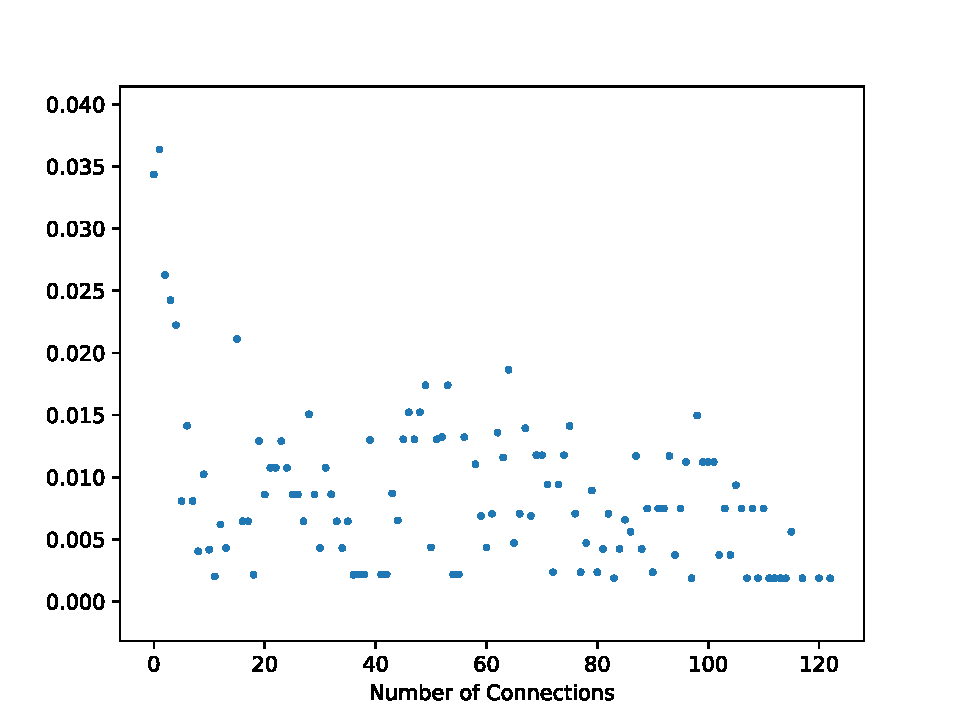
\includegraphics[scale=0.50,trim={0 0 1cm 1cm},clip]{./Figures/DD/caDataCOEDD.pdf}}
\end{minipage}
\caption[Average Degree Distribution in \textit{Xenopus} Calcium Imaging Data Predictions]{\textbf{Average Degree Distribution in \textit{Xenopus} Calcium Imaging Data Predictions.} (a) The average degree distribution of the resulting variable activation model prediction adjacency matrix from 6 \textit{in-vivo} recordings of calcium imaging data from {Xenopus Laevis} (b) Distribution of the adjacency matrices produced from the base model, from the same datasets as (a).}
\label{fig:DD2}
\end{figure}

\begin{figure}[H]
\vspace*{-5mm}
\begin{minipage}{0.49\linewidth}
\captionsetup{position=top}
\subfloat[]{\label{DD:a}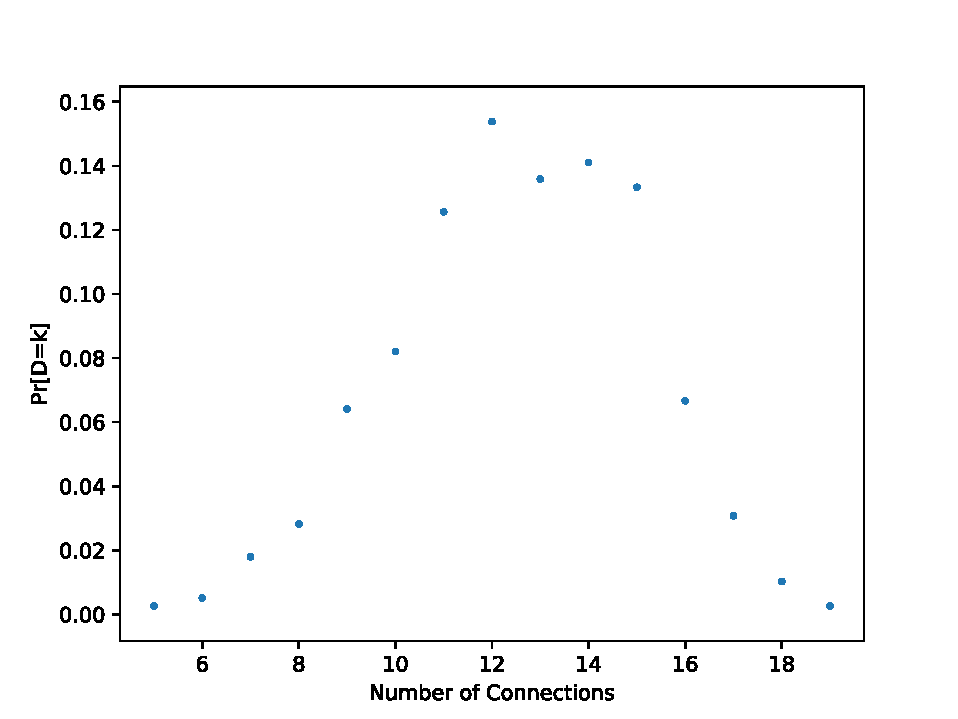
\includegraphics[height=5cm,scale=0.45,trim = {0 0.3cm 1cm 1.2cm},clip]{./Figures/DD/simulatedvarDDPop10.pdf}}
\end{minipage}
\begin{minipage}{0.50\linewidth}
\captionsetup{position=top}
\subfloat[]{\label{DD:b}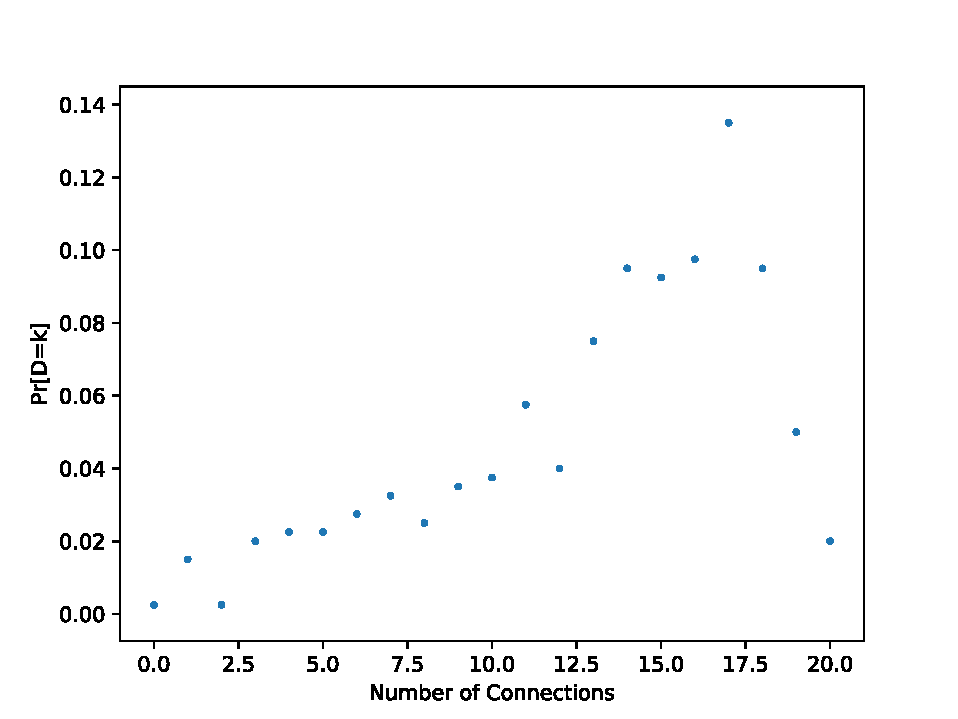
\includegraphics[height=5cm,scale=0.45,trim={0 0.3cm 1cm 1.2cm},clip]{./Figures/DD/simulatedCOEDDPop10.pdf}}
\end{minipage}
\vspace*{-5mm}
\begin{minipage}{0.49\linewidth}
\captionsetup{position=top}
\subfloat[]{\label{DD:c}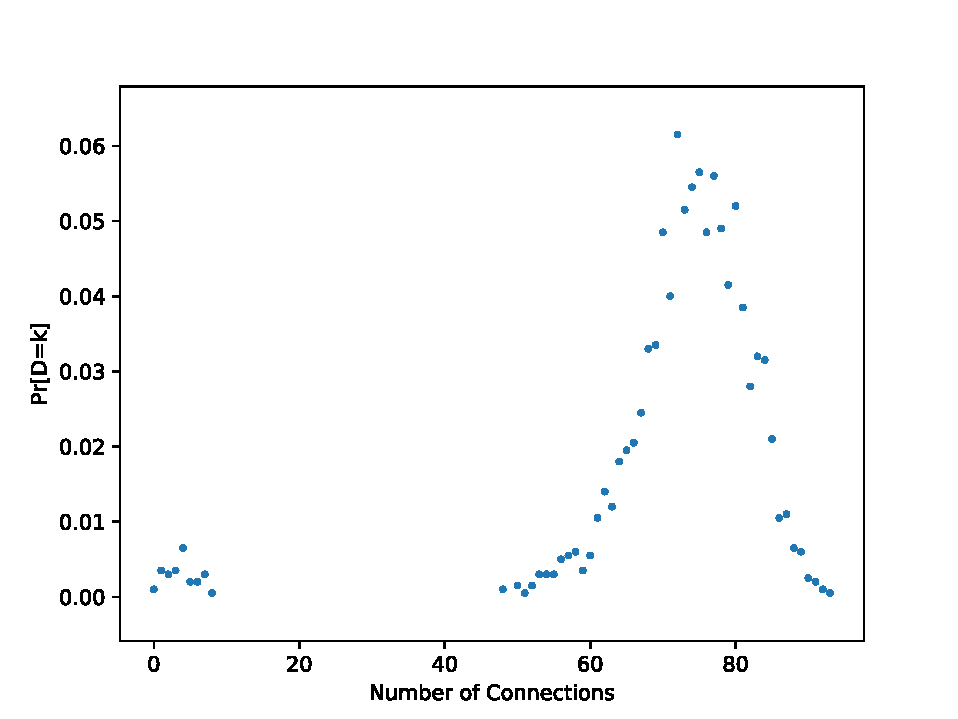
\includegraphics[height=5cm,scale=0.45,trim={0 0.3cm 1cm 1.2cm},clip]{./Figures/DD/simulatedvarDDPop50.pdf}}
\end{minipage}
\begin{minipage}{0.50\linewidth}
\captionsetup{position=top}
\subfloat[]{\label{DD:d}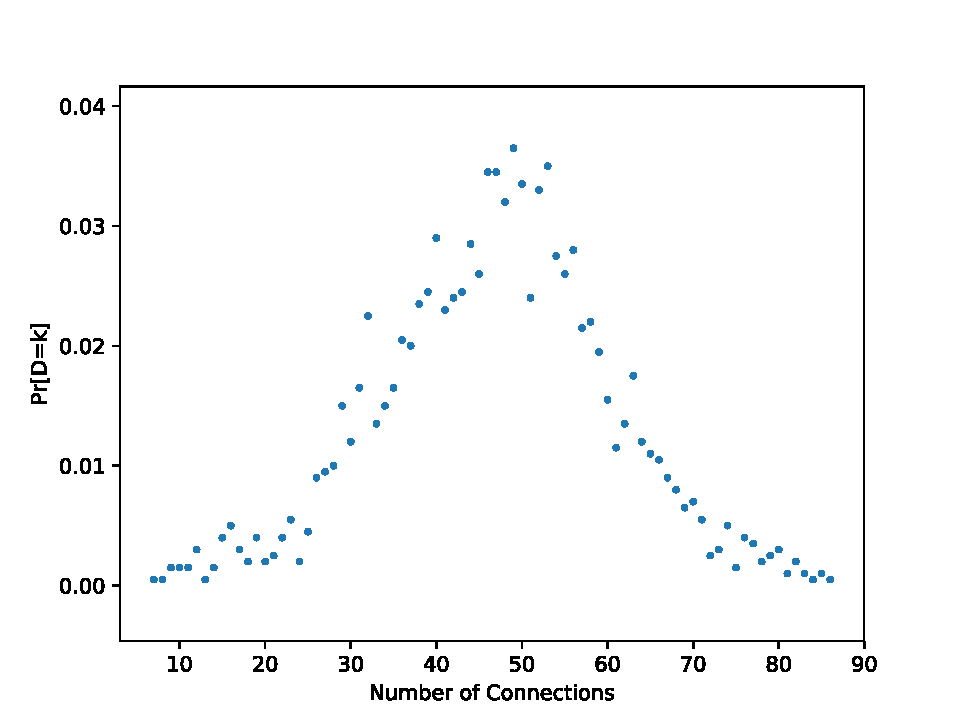
\includegraphics[height=5cm,scale=0.45,trim={0 0.3cm 1cm 1.2cm}, clip]{./Figures/DD/simulatedCOEDDPop50.pdf}}
\end{minipage}
\vspace*{-5mm}
\begin{minipage}{0.49\linewidth}
\captionsetup{position=top}
\subfloat[]{\label{DD:e}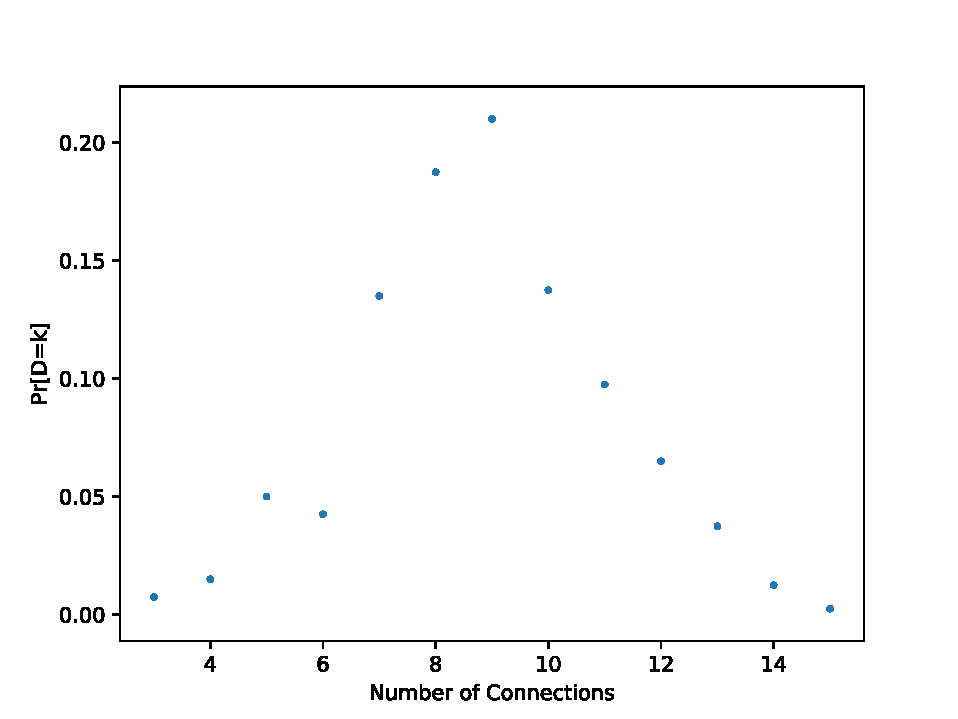
\includegraphics[height=5cm,scale=0.45,trim={0 0.3cm 1cm 1.2cm}, clip]{./Figures/DD/gtPop10.pdf}}
\end{minipage}
\begin{minipage}{0.50\linewidth}
\captionsetup{position=top}
\subfloat[]{\label{DD:f}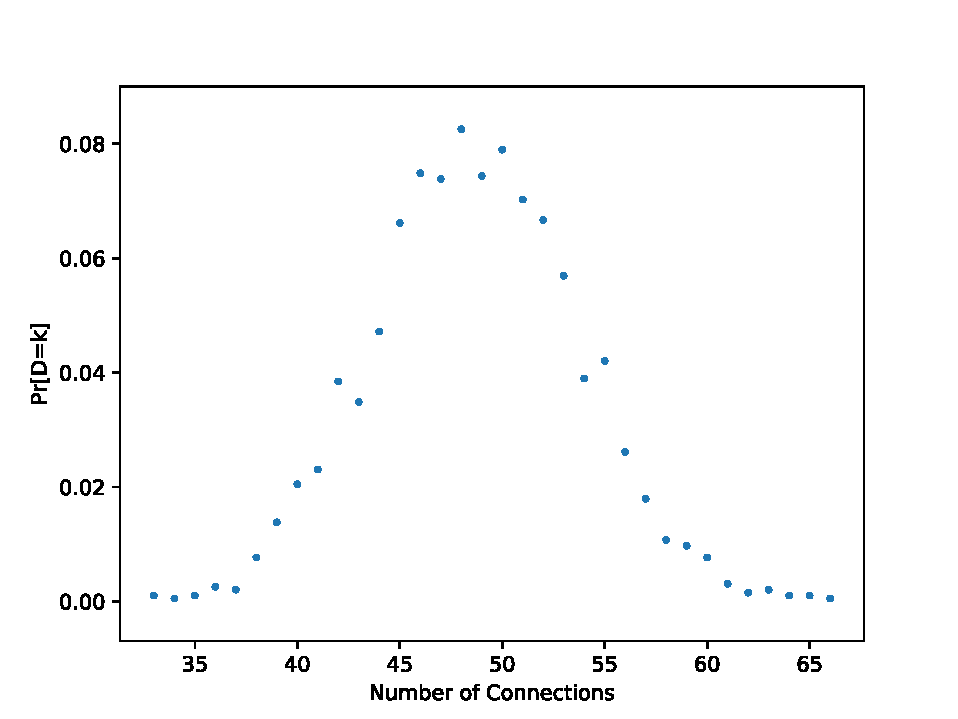
\includegraphics[height=5cm,scale=0.45,trim={0 0.3cm 1cm 1.2cm}, clip]{./Figures/DD/gtPop50.pdf}}
\end{minipage}

\caption[Average Degree Distribution in Simulated Data Predictions]{\textbf{Average Degree Distribution in Simulated Data Predictions.} (a)Average degree distribution of the simulated data from population size 10, averaged across the resulting adjacency matrices of the variable activation function model across 40 simulated spike time matrices.(b)Average degree distribution from base model. (c) Average degree distribution of the simulated data from population size 50, averaged across the resulting adjacency matrices of the variable activation function model produced from 40 simulated spike time matrices.(d) Average degree distribution of the simulated data from population size 50, averaged across predictions from the base model produced from 40 simulated spike time matrices.(e)(f) Calculated average degree distributions across 40 randomly generated networks of population size 10 and 50, respectively.}
\label{fig:DD}
\end{figure}

\subsection{ROC}
The receiver operating characteristic (ROC) curve is a measure of performance for testing the accuracy of models where the ground truth underlying the data is available for comparison. The receiver operating characteristic plots the true positive rate (TPR) against the false positive rate (FPR) to evaluate the performance of the model on the simulated data sets (Garofalo et al., 2009). The TPR is evaluated according to $$TPR = \frac{TP}{TP + FN}$$ where the FPR is evaluated according to $$FPR = \frac{FP}{FP + TN}$$ where TP, FP, TN and FN are defined in the contingency table (Figure \ref{contingencyTable})

\begin{figure}[H]
\centering
\begin{tabular}{|l|l|l|l|}
\hline
                                     & \multicolumn{3}{l|}{True Condition} \\ \hline
\multirow{3}{*}{Predicted Condition} &            & Positive   & Negative  \\ \cline{2-4} 
                                     & Positive   & TP         & FP        \\ \cline{2-4} 
                                     & Negative   & FN         & TN        \\ \hline
\end{tabular}
\caption[Contingency Table]{Contingency Table. The designations of true positive (TP), false positive (FP), false negative (FN), and true negative (TN). For example, a positive appearing in the true condition and a positive appearing in the predicted condition is a TP.}
\label{contingencyTable}
\end{figure}
In the adjacency matrices, positives are defined as a value of "1" and negative as "0". When comparing between two matrices, a positive in the predicted matrix at $P_{ij}$ and a positive in the ground truth matrix at $M_{ij}$ indicate a true positive. TPRs and FPRs are calculated for cross-correlation, the base model, and the variable activation function model.\par
ROC curves are constructed by varying some parameter and observing the resulting TPRs and FPRs. In the ROC curve below, we simply increase the threshold at which a normalized value in the predicted weight matrix is counted as a connection. Starting from a threshold of 0, which allows all possible connections, we increase by 0.01 at every iteration, until 1, at which point there are no longer any connections in the predicted matrix. At every threshold, the TPRs and FPRs are calculated. In the case of the base model and the activation function model, the TPRs and FPRs at every threshold are calculated for 40 distinct datasets on which the models were trained. The TPRs and FPRs for every dataset, at every threshold, is accumulated. Redundant TPR and FPR calculations are removed before plotting and analysis; plotting the redundant points would result in overlapping points and a weighted area under the curve (AUC). ROC curves for models are plotted against random guessing, represented as a linear relationship between TPR and FPR, with an AUC of 0.5. Cross-correlation ROC is calculated across 100 distinct simulated datasets, with TPR and FPR accumulated across all datasets and redundant TPR and FPR calculations removed.\par

\begin{figure}[H]
\begin{minipage}{0.49\linewidth}
\captionsetup{position=top}
\subfloat[]{\label{roc:a}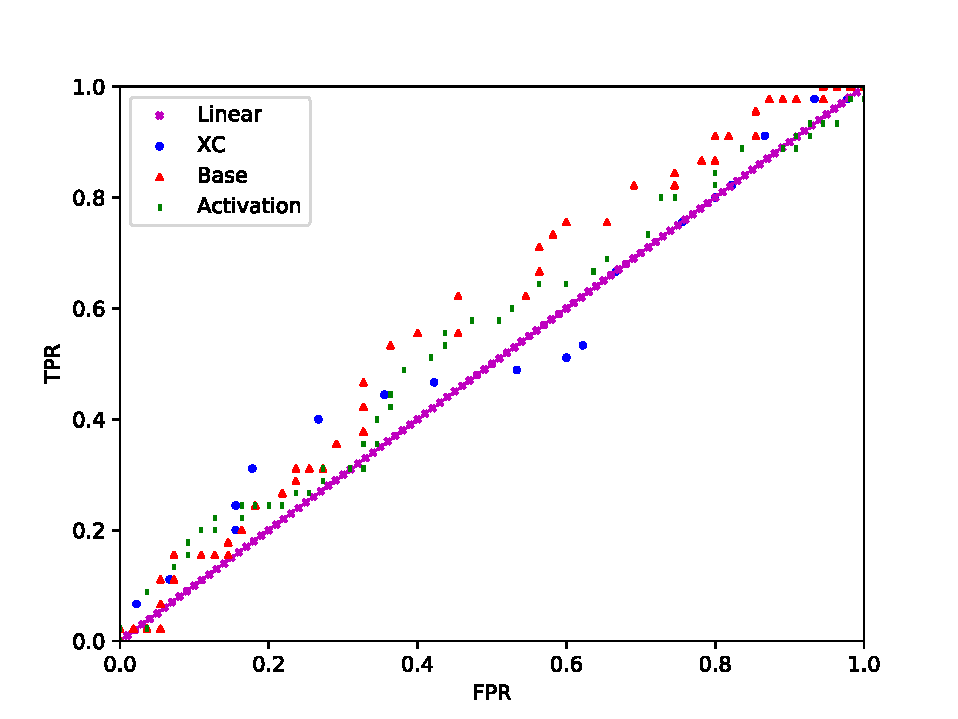
\includegraphics[scale=0.5,trim={0 0 1cm 0},clip]{./Figures/rocPop10.pdf}}
\end{minipage}
\begin{minipage}{0.50\linewidth}
\captionsetup{position=top}
\subfloat[]{\label{roc:b}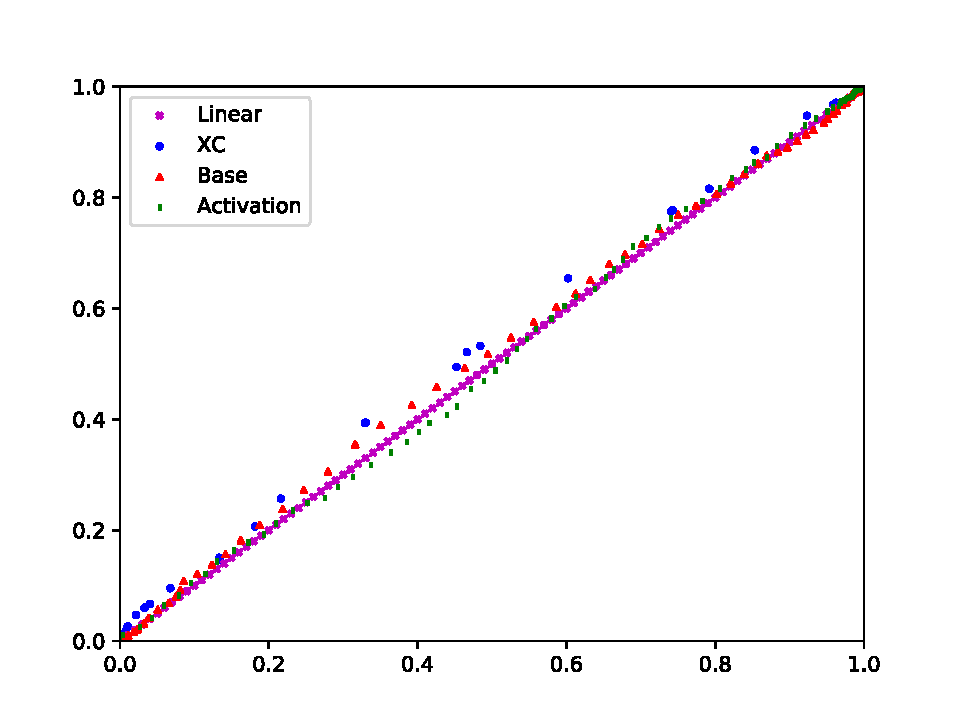
\includegraphics[scale=0.5,trim={0 0 1cm 0},clip]{./Figures/rocPop50.pdf}}
\end{minipage}
\caption[Receiver Operating Characteristic]{Receiver Operating Characteristic. The linear function depicted is random guessing, with an AUC of 0.5.(a) ROC on cross-correlations and model results from population size of 10. Activation AUC = 0.54, Base = 0.58, XC = 0.53. (b) ROC on cross-correlations and model results from population size of 50. Activation AUC = 0.49, Base = 0.51, XC = 0.53. Activation is the variable activation function model, while Base is the base model.}
\label{fig:roc}
\end{figure}

To better compare the curves, we calculate the AUC to describe the curve as a single value. The AUC is calculated as the integral of the ROC curve from 0 to 1, using the composite trapezoidal rule. The accumulated ROC curves depicted in \ref{fig:roc} have the calculated AUC as listed in the caption. The average AUCs, where an ROC curve and AUC are individually calculated for each dataset and averaged, are as follows: XC = 0.46 ($\pm$ .07), Activation AUC = 0.45 ($\pm$ .09), Base AUC = 0.47 ($\pm$ .09) for population size 10, and XC = .48 ($\pm$ .01), Activation AUC = 0.44 ($\pm$ .02), Base AUC 0.49 ($\pm$ .01) for population size 50. These values are calculated differently from the the values listed in \ref{fig:roc}, and is slightly lower average AUC, indicating that the model performs approximately as well as random guessing when testing for accuracy of prediction on the underlying ground truth matrix of the simulated data.

\newpage
\section{Discussion}

\subsection{Differences in Degree Distribution}
The calculated average degree distributions of the simulated data resemble a Gaussian distribution in the cases of both models, most clearly seen in Figures \ref{DD:c} and \ref{DD:d}. The ground truth degree distributions displayed in Figures \ref{DD:e} and \ref{DD:f} are randomly generated networks, with each network generated in the same fashion as the ground truth matrices for all network simulations. While the predicted degree distribution for population size 10 from the base model is right-skewed (\ref{DD2:b}), all other distributions resemble the binomially distributed probabilities. In the degree distributions produced from \textit{Xenopus} calcium imaging data, the curves do not resemble the Gaussian distribution; in both cases, the distributions resemble a power-law behavior, characterized by the higher rate of sparsely connected nodes, and the lower rate of densely connected nodes (Hernandez and Meigem, 2011; Massobrio et al., 2015). As described in section \ref{sssec:NM}, the power-law behavior defines a scale-free network (Eyton and Marom, 2006; Massobrio et al., 2015). This distinct connection pattern differs from that of networks that fit a Gaussian distribution, where nodes in the network tend to have a number of connections varying around an average number of connections.\par
While the degree distribution does not inform us about the exact manner in which the neurons in the network are connected, the distribution indicates that the model may be able to capture underlying patterns of connectivity in the population. However, whether or not the underlying connectivity pattern of neurons fits a power-law distribution is a debated topic among the neuroscience community. Some studies have indicated scale-free architectures in networks, such as in \textit{in-vitro} cortical neuronal networks (Eyton and Moran, 2006), in rat hippocampal slices (Bonifazi et al., 2009) and in other studies of network reconstruction (Pajevic and Plenz, 2009). Additionally, a study in the \textit{Xenopus} optic tectum indicates the scale-free acrhictecture to be a possibility; however, in this particular study, the researchers found a uniformly distributed network to be a more robust, and therefore more likely architecture. Other studies find no evidence of scale-free architectures (Stetter et al., 2012).

\subsection{Model Error Convergence}
When the model is run on two time steps, we observe distinct error convergence patterns, dependent on the activity of the input and target time steps. As observed in Figures \ref{errorTwoTime:a} and \ref{errorTwoTime:c}, the error convergence of an input spike time step containing a single spike and a target spike time step containing a single spike converges at around 20 iterations of training in the base model, and around 45 iterations of training in the variable activation function model. Furthermore, the error convergence between ten runs results in a low standard deviation. Training the model on distinct spiking patterns results in larger standard deviations; the stable standard deviations indicate that, between all distinct spiking patterns, the model generally converged at the same iteration, at widely differing values of convergence, indicating different calculations of error dependent on the spiking pattern.

\subsection{Receiver Operating Characteristic and Accuracy of Model}
The receiver operating characteristic curve is a metric for evaluating performance accuracy of a model. Here, we observe the ROC of performance on our cross-correlation implementation, our base model, and our variable activation function model. While the initial ROC curve of the base and activation modles with a population size 10 (figure \ref{roc:a}) appeared to perform better then the implementation of cross-correlation, the cross-correlation method performed worse than implementations of cross-correlation applied in other studies, as well as methods such as mutual information, transfer entropy applied in other studies (Garofalo et al., 2009; Stetter et al., 2012). Additionally, while the AUC calculated from averaging TPRs and FPRs across all cross-correlation results (AUC = 0.53) is higher than the linear relationship (AUC = 0.5), the average AUC calculated by determining individual AUC and averaging is slightly lower (AUC = 0.46 ($\pm$ .07)). These results indicate that the base model, variable activation function model, and the cross-correlation implementation here did not perform better than any existing method applied in other studies, where cross-correlation AUC = 0.70 ($\pm$ 0.05).

\clearpage
\section{Conclusion and Future Work}
We develop a model based on methods applied in neural networks, an architecture used in machine learning, and attempt to extract the underlying connectivity of the populations of neurons by training the model on the spike-time data of these populations. While the results suggest that the model is able to capture the degree distributions of the underlying networks, the model is not able to accurately predict the connections of the population.\par
Due to technical limitations, analysis of calcium imaging data was performed on a sample size of 6 spike time datasets. Analysis on a larger sample size would solidify the findings of the degree distribution presented in Figure \ref{fig:DD2}, and allow for a more accurate comparison with the degree distributions random networks characterized in Figure \ref{fig:DD}. Alternatively, testing the model on simulated data from a scale-free network and analyzing the underlying degree distribution would validate the findings presented here.\par
	There are various possible improvements that could be made to the model. Here, we use an architecture resembling a simplified neural network, with changes to the update sequence to allow each neuron a unique activation function resembling the logistic function. Furthermore, we restrict the network to a single set of weights between the input and output layers, constraining the learning capabilities of the network. One possibility for improvement is inclusion of backpropagation methods that incorporate the timing of the spike (Bohte et al., 2002; Werbos, 1990). Such backpropagation methods are more biologically inspired than traditional neural networks; these methods are inspired by the temporal coding activity of neurons, where information is conveyed in the precise timing of a spike (Purves, 2004, 349; Bohte et al., 2002). Improving the model to account for further network dynamics of neurons would likely produce more accurate reconstructions.\par


\clearpage
\section{Supplementary Material}
\subsection{Code and Data}
All code and and data are available on github at https://github.com/DerekLow18/SPROJ.git.
\subsection{Supplementary Figure}
\begin{figure}[H]
\begin{minipage}{0.49\linewidth}
\captionsetup{position=top}
\subfloat[]{\label{QQ:a}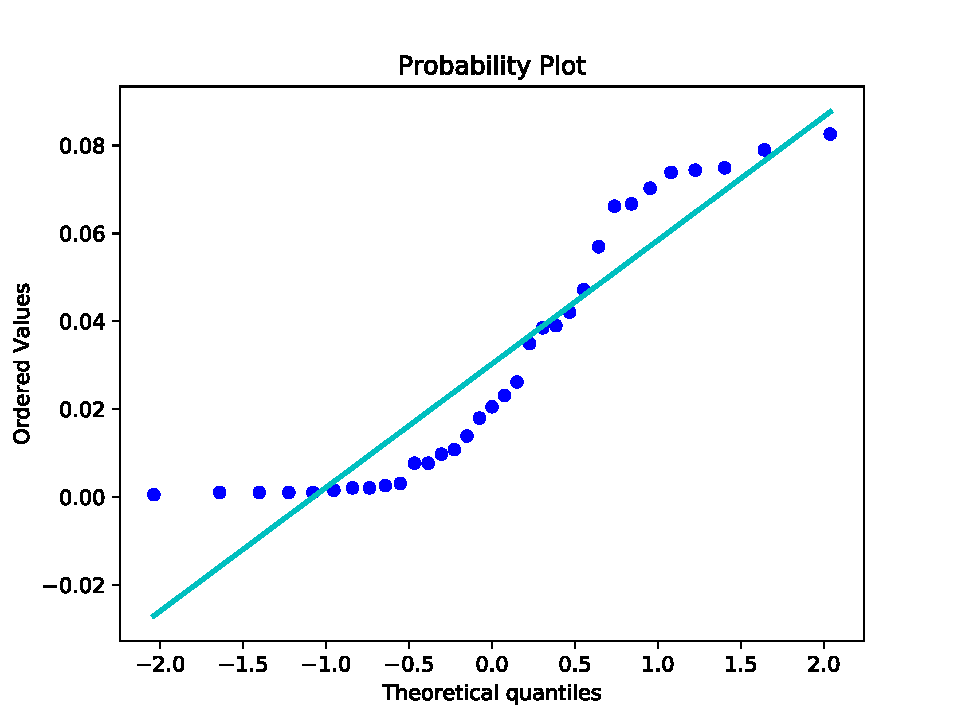
\includegraphics[scale=0.5,trim={0 0 1cm 0.5cm},clip]{./Figures/DD/gtQQpop50.pdf}}
\end{minipage}
\begin{minipage}{0.50\linewidth}
\captionsetup{position=top}
\subfloat[]{\label{QQ:b}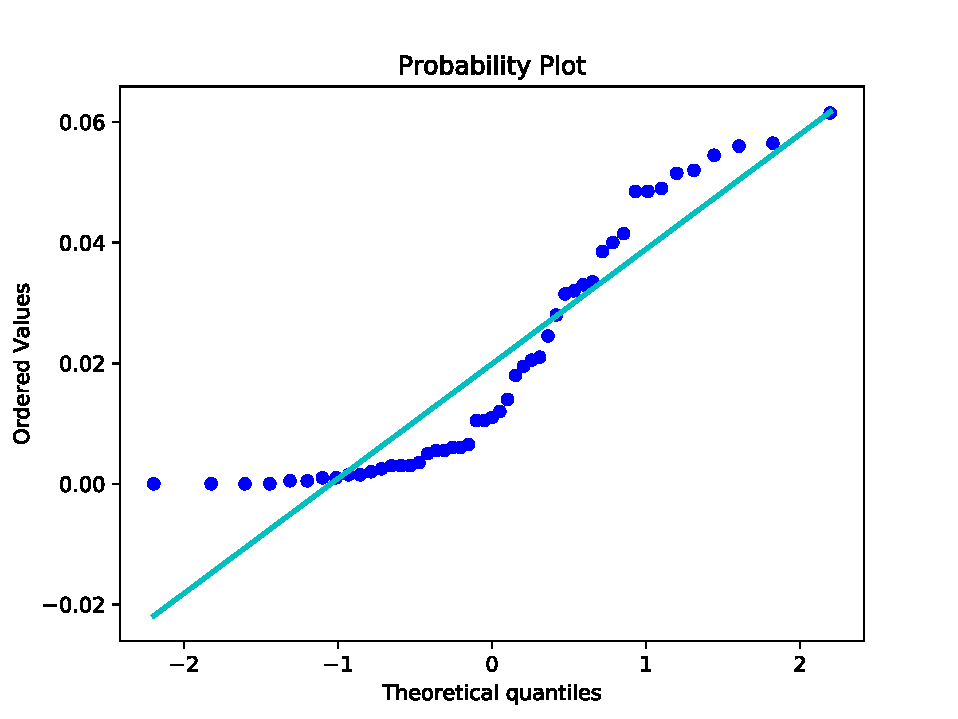
\includegraphics[scale=0.5,trim={0 0 1cm 0.5cm},clip]{./Figures/DD/simulatedvarQQpop50.pdf}}
\end{minipage}
\caption[(S1) Q-Q Plots of Degree Distributions]{\textbf{Q-Q Plots of Degree Distributions.} Here, we compare the average degree distribution of (a) 40 ground truth adjacency matrices of population size 50 ($R^2$ = 0.9329), and (b) 40 predicted adjacency matrices of population size 50 ($R^2$ = 0.9299), to the normal distribution.}
\label{fig:QQ}
\end{figure}

\clearpage
\section{Works Cited}
%\bibliographystyle{plain}
%\bibliography{references}
\begin{spacing}{1}
\begin{enumerate}
\item Alberts B, Johnson A, Lewis J, et al. Molecular Biology of the Cell. 4th edition. New York: Garland Science; 2002. Ion Channels and the Electrical Properties of Membranes. Available from: https://www.ncbi.nlm.nih.gov/books/NBK26910/
\item Armstrong, C. M., \& Hille, B. (1998). Voltage-Gated Ion Channels Review and Electrical Excitability Early Biophysics and Voltage Clamp Revealed Voltage-Gated Membrane Permeabilities. Neuron, 20, 371–380.\\ https://doi.org/10.1016/S0896-6273(00)80981-2
\item Bean, B. P. (2007). The action potential in mammalian central neurons. Nature Reviews Neuroscience, 8(6), 451–465. https://doi.org/10.1038/nrn2148
\item Berridge, M. J., Lipp, P., \& Bootman, M. D. (2000). The Versatility and Universality of Calcium Signalling. Nature Review Molecular Cell Biology, 1(October), 11–21.
\item Biswal, B., Yetkin, F. Z., Haughton, V. M., \& Hyde, J. S. (1995). Functional Connectivity in the Motor Cortex of Resting. Magnetic Resonance in Medicine, 34(4), 537–541.
\item Bock, D. D., Lee, W. A., Kerlin, A. M., Andermann, M. L., Hood, G., Wetzel, A. W., … Reid, R. C. (2011). Network anatomy and in vivo physiology of visual cortical neurons. Nature, 471(7337), 177–182. https://doi.org/10.1038/nature09802
\item Bohte, S. M., Kok, J. N., \& Poutrã, H. La. (2002). Error-backpropagation in temporally encoded networks of spiking neurons. Neurocomputing, 48, 17–37.
\item Bonifazi, P., Goldin, M., Picardo, M. A., Jorquera, I., Cattani, A., Bianconi, G., … Cossart, R. (2009). GABAergic hub neurons orchestrate synchrony in developing hippocampal networks. Science, 326(5958), 1419–1424. https://doi.org/10.1126/science.1175509
\item Bottou, L. (1991). Stochastic Gradient Learning in Neural Networks. Proceedings of Neuro-Nimes, EC2.
\item Bottou, L. ,Curtis, F. E. \& Nocedal J. (2018). Optimization methods for largescale
machine learning. arXiv:1606.04838v3.
\item Brette, R. (2015). What Is the Most Realistic Single-Compartment Model of Spike Initiation? PLoS Computational Biology. https://doi.org/10.1371/journal.pcbi.1004114
\item Brette, R., Rudolph, M., Carnevale, T., Hines, M., Beeman, D., Bower, J. M., … Muller, E. (2007). Simulation of networks of spiking neurons: A review of tools and strategies. J Comput Neurosci, 23(3), 349–398. https://doi.org/10.1007/s10827-007-0038-6
\item Carrillo-Reid, L., Yang, W., Bando, Y., Peterka, D. S., \& Yuste, R. (2016). Imprinting Cortical Ensembles. Science, 353(6300), 691–694. https://doi.org/10.1126/science.aaf7560
\item Costa, L. da F., Rodrigues, F. A., Travieso, G., \& Boas, P. R. V. (2005). Characterization of complex networks: A survey of measurements. Advances in Physics, 56(1), 167–242. https://doi.org/10.1080/00018730601170527
\item Denk, W., Strickler, J. H., \& Webb, W. W. (1990). Two-Photon Laser Scanning Fluorescence Microscopy. Science, 248(4951), 73–76.
\item Dong, W., Lee, R. H., Xu, H., Yang, S., Pratt, K. G., Cao, V., … Aizenman, C. D. (2008). Visual Avoidance in Xenopus Tadpoles Is Correlated With the Maturation of Visual Responses in the Optic Tectum. Journal of Neurophysiology, 101(2), 803–815.\\https://doi.org/10.1152/jn.90848.2008
\item Eytan, D., \& Marom, S. (2006). Dynamics and Effective Topology Underlying Synchronization in Networks of Cortical Neurons. Journal of Neuroscience, 26(33), 8465–8476. \\https://doi.org/10.1523/JNEUROSCI.1627-06.2006
\item Garofalo, M., Nieus, T., Massobrio, P., \& Martinoia, S. (2009). Evaluation of the Performance of Information Theory- Based Methods and Cross-Correlation to Estimate the Functional Connectivity in Cortical Networks. PLoS ONE, 4(8).\\https://doi.org/10.1371/journal.pone.0006482
\item Grady, C. L., McIntosh, A. R., \& Craik, F. I. M. (2003). Age-related differences in the functional connectivity of the hippocampus during memory encoding. Hippocampus, 13(5), 572–586. https://doi.org/10.1002/hipo.10114
\item Grienberger, C., \& Konnerth, A. (2012). Imaging Calcium in Neurons. Neuron. \\https://doi.org/10.1016/j.neuron.2012.02.011
\item Grynkiewicz, G., Poenie, M., and Tsien, R.Y. (1985). A new generation of Ca 2+ indicators with greatly improved fluorescence properties. J. Biol. Chem.260 , 3440–3450
\item Gurney, K. An Introduction to Neural Networks. London: Taylor \& Francis, 2004.
\item Hamm, J. P., Peterka, D. S., Gogos, J. A., \& Yuste, R. (2017). Altered Cortical Ensembles in Mouse Models of Schizophrenia. Neuron, 94(1), 153–167.e8\\https://doi.org/10.1016/j.neuron.2017.03.019
\item Hastie T., Tibshirani R., Friedman J. (2009) Overview of Supervised Learning. In: The Elements of Statistical Learning. Springer Series in Statistics. Springer, New York, NY
\item Haydon, P. G. (2001). Glia : Listening and Talking To The Synapse. Nature Reviews Neuroscience, 2(March), 186–193.
\item Hecht-Nielsen, R. (1989). Theory of the Backpropagation Neural Network. Proceedings Of The International Joint Conference On Neural Networks, 1, 593–605.\\https://doi.org/10.1109/IJCNN.1989.118638
\item Hernández, J. M., \& Mieghem, P. Van. (2011). Classification of graph metrics. Delft University of Technology.
\item Hodgkin, A. L., \& Kats, B. (1949). The Effect of Sodium Ions on the Electrical Activity of the Giant Axon of the Squid. The Journal Of Physiology, 108(1), 37–77.
\item Hoffman, D. A., Magee, J. C., Colbert, C. M., \& Johnston, D. (1997). K + channel regulation of signal propagation in dendrites of hippocampal pyramidal neurons. Nature, 387(June), 869–876.
\item Izhikevich, E. M. (2004). Which model to use for cortical spiking neurons? IEEE Transactions on Neural Networks. https://doi.org/10.1109/TNN.2004.832719
\item Jang, E. V., Ramirez-Vizcarrondo, C., Aizenman, C. D., \& Khakhalin, A. S. (2016). Emergence of Selectivity to Looming Stimuli in a Spiking Network Model of the Optic Tectum. Frontiers in Neural Circuits, 10(November), 1–14. https://doi.org/10.3389/fncir.2016.00095
\item Kalman, R. E. (1960). A New Approach to Linear Filtering and Prediction Problems. Journal of Basic Engineering, 82(1), 35. https://doi.org/10.1115/1.3662552
\item Katz, B., \& Miledi, R. (1967). A Study of Synaptic Transmission in the Absence of Nerve Impulses. Department of Biophysics, University College London, 407–436.
\item Katz, B., \& Miledi, R. (1968). The role of calcium in neuromuscular facilitation. Journal of Physiology, 195, 481–492. https://doi.org/10.1111/j.1365-3040.1992.tb01004.x
\item Khakhalin, A. S., Koren, D., Gu, J., Xu, H., \& Aizenman, C. D. (2014). Excitation and inhibition in recurrent networks mediate collision avoidance in Xenopus tadpoles. European Journal of Neuroscience, 40(6), 2948–2962. https://doi.org/10.1111/ejn.12664
\item Knox, C. K. (1981). Detection of neuronal interactions using correlation analysis. Trends in Neurosciences, 4(C), 222–225. https://doi.org/10.1016/0166-2236(81)90070-9
\item Kunkel, Susanne, Morrison, Abigail, Weidel, Philipp, Eppler, Jochen Martin, Sinha, Ankur, Schenck, Wolfram, … Plesser, Hans Ekkehard. (2017, March 1). NEST 2.12.0. Zenodo. http://doi.org/10.5281/zenodo.259534
\item Marblestone, A., Wayne, G., \& Kording, K. (2016). Towards an integration of deep learning and neuroscience. https://doi.org/10.3389/fncom.2016.00094
\item Massobrio, P., Pasquale, V., \& Martinoia, S. (2015). Self-organized criticality in cortical assemblies occurs in concurrent scale-free and small-world networks. Nature Publishing Group, (October 2014), 1–16. https://doi.org/10.1038/srep10578
\item McCulloch, W. S., \& Pitts, W. H. (1943). A Logical Calculus of the Ideas Immanent In Nervous Activity. Bulletin of Mathematical Biophysics, 5, 115–133.
\item Miller, E. K., \& Cohen, J. D. (2001). An Integrative Theory of Prefrontal Cortex Function. Annual Review of Neuroscience, 24, 167–202.
\item Minshew, N. J., \& Williams, D. L. (2007). The New Neurobiology of Autism: Cortex, Connectivity, and Neuronal Organization. Archives of Neurology, 64(7), 945–950.
\item Mitchell, M. (1996). An Introduction to Genetic Algorithms (5th ed.). Cambridge, MA.: MIT Press.
\item Ntziachristos, V. (2010). Going deeper than microscopy : the optical imaging frontier in biology. Nature Publishing Group, 7(8), 603–614. https://doi.org/10.1038/nmeth.1483
\item Orrenius, S., Zhivotovsky, B., \& Nicotera, P. (2003). Regulation of Cell Death: The Calcium - Apoptosis Link. Nature Review Molecular Cell Biology, 4(July), 552–565.\\ https://doi.org/10.1038/nrm1150
\item Pajevic, S., \& Plenz, D. (2009). Efficient network reconstruction from dynamical cascades identifies small-world topology of neuronal avalanches. PLoS Computational Biology, 5(1). https://doi.org/10.1371/journal.pcbi.1000271
\item Pandarinath, C., Shea, D. J., Collins, J., Jozefowicz, R., Stavisky, S. D., Kao, J. C., … Sussillo, D. (2017). Inferring single-trial neural population dynamics using sequential auto-encoders. bioRxiv.\\Retrieved from http://biorxiv.org/content/early/2017/06/20/152884.abstract
\item Paredes, R. M., Etzler, J. C., Watts, L. T., Zheng, W., \& Lechleiter, J. D. (2008). Chemical calcium indicators. Methods, 46(3), 143–151. https://doi.org/10.1016/j.ymeth.2008.09.025
\item Porro, C. A., Francescato, M. P., Cettolo, V., Diamond, M. E., Baraldi, P., Zuiani, C., … Prampero, P. E. (1996). Primary Motor and Sensory Cortex Activation during Motor Performance and Motor Imagery : A Functional Magnetic Resonance Imaging Study. The Journal of Neuroscience, 16(23), 7688–7698.
\item Purves, D., Augustine, G. J., Fitzpatrick, D., Hall, W. C., LaMantia, A., and White, L. E. (2012). Neuroscience. Sunderland, Massachusetts.: Sinauer Associates, Inc.
\item Rakic, P. (2006). Evolution of the neocortex. Current Biology, 16(21), 910–914. \\https://doi.org/10.1038/nrn2719.Evolution
\item Robbins, H., \& Monro, S. (1951). A Stochastic Approximation Method. The Annals of Mathematical Statistics, 22(3), 400–407.
\item Rubinov, M., \& Sporns, O. (2010). Complex network measures of brain connectivity: Uses and interpretations. NeuroImage, 52, 1059–1069.\\ https://doi.org/10.1016/j.neuroimage.2009.10.003
\item Ruder, S. (2016). An overview of gradient descent optimization algorithms.\\ arXiv:1609.04747v2, 1–14.
\item Stetter  O,  Battaglia  D,  Soriano  J,  Geisel  T  (2012)  Model-Free  Reconstruction  of  Excitatory  Neuronal  Connectivity  from  Calcium  Imaging  Signals.  PLo S Comput  Biol  8(8):  e1002653. doi:10.1371/journal.pcbi.1002653
\item Shimomura, O., Johnson, F. H. and Saiga, Y. (1962), Extraction, Purification and Properties of Aequorin, a Bioluminescent Protein from the Luminous Hydromedusan, Aequorea. J. Cell. Comp. Physiol., 59: 223–239. doi:10.1002/jcp.1030590302
\item Sporns, O., Chialvo, D., Kaiser, M., and Hilgetag, C. (2004). Organization, development and function of complex brain networks. Trends in Cognitive Sciences, 8(9), 418-425. \\doi:10.1016/j.tics.2004.07.008
\item Stam, C. J. (2014). Modern network science of neurological disorders. Nature Reviews Neuroscience, 15(10), 683–695. https://doi.org/10.1038/nrn3801
\item Steels, L. (2007). Fifty Years of AI: From Symbols to Embodiment -and Back, 18–28.
\item Stetter, O., Battaglia, D., Soriano, J., and Geisel, T. (2012). Model-Free Reconstruction of Excitatory Neuronal Connectivity from Calcium Imaging Signals. PLoS Computational Biology. https://doi.org/10.1371/journal.pcbi.1002653
\item Strogatz, S. H. (2001). Exploring complex networks. Nature, 410(6825), 268–276.\\https://doi.org/10.1038/35065725
\item Svoboda, K., Yasuda, R., \& Carolina, N. (2006). Principles of Two-Photon Excitation Microscopy and Its Applications to Neuroscience. Neuron, 50, 823–839.\\https://doi.org/10.1016/j.neuron.2006.05.019
\item Terry, R. D., Masliah, E., Salmon, D. P., Butters, N., Deteresa, R., Hill, R., … Katzman, R. (1991). Physical Basis of Cognitive Alterations in Alzheimer ’ s Disease : Synapse h s s Is the Major Correlate of Cognitive Impairment. Annals of Neurology, 30(4), 572–580.
\item Tetzlaff, C., Okujeni, S., Egert, U., Wörgötter, F., \& Butz, M. (2010). Self-organized criticality in developing neuronal networks. PLoS Computational Biology, 6(12).\\https://doi.org/10.1371/journal.pcbi.1001013
\item Turing, A. M. (2009). Computing machinery and intelligence. In Parsing the Turing Test: Philosophical and Methodological Issues in the Quest for the Thinking Computer.\\https://doi.org/10.1007/978-1-4020-6710-5\_3
\item Werbos, P. J. (1990). Backpropagation Through Time: What It Does and How to Do It. Proceedings of the IEEE, 78(10), 1550–1560. https://doi.org/10.1109/5.58337
\item Widrow, B., \& Lehr, M. A. (1990). 30 Years of Adaptive Neural Networks: Perceptron, Madaline, and Backpropagation. Proceedings of the IEEE, 78(9), 1415–1442.\\https://doi.org/10.1109/5.58323
\item Vogelstein, J. T., Packer, A. M., Machado, T. A., Sippy, T., Babadi, B., Yuste, R., \& Paninski, L. (2010). Fast Nonnegative Deconvolution for Spike Train Inference From Population Calcium Imaging. Journal of Neurophysiology, 104(6), 3691–3704.\\ https://doi.org/10.1152/jn.01073.2009
\item Xu, H., Khakhalin, A. S., Nurmikko, A. V., \& Aizenman, C. D. (2011). Visual Experience-Dependent Maturation of Correlated Neuronal Activity Patterns in a Developing Visual System. Journal of Neuroscience, 31(22), 8025–8036.\\ https://doi.org/10.1523/JNEUROSCI.5802-10.2011
\item Zhou, D., Xiao, Y., Zhang, Y., Xu, Z., \& Cai, D. (2014). Granger causality network reconstruction of conductance-based integrate-and-fire neuronal systems. PLoS ONE, 9(2). https://doi.org/10.1371/journal.pone.0087636
\item Zucker, R. S. (1989). Short-term synaptic plasticity. Annual Review of Neuroscience, 12, 13–31.
\item Zucker, R. S. (1999). Calcium- and activity-dependent synaptic. Current Opinion in Neurobiology, 9(3), 305–313.
\end{enumerate}
\end{spacing}
\end{document}
